\documentclass[12pt,halfline,a4paper]{ouparticle}
\usepackage{tabularx}
\usepackage{graphicx}

\begin{document}

\title{Sample Article for\break {Oxford University Press~Journals}}

\author{%
\name{Lucas Reeh}
\email{lreeh@student.tugraz.at}
}
\date{\today}

\keywords{computational intelligence, assignement1}

\begin{titlepage}
   \begin{center}
     \begin{huge}
		   %% Update assignment number here
           \textbf{Assignment 1}
     \end{huge}
   \end{center}

   \begin{center}
     \begin{large}
           Computational Intelligence, SS2017
     \end{large}
   \end{center}

   \begin{center}
 \begin{tabularx}{\textwidth}{|>{\hsize=.33\hsize}X|>{\hsize=.33\hsize}X|>{\hsize=.33\hsize}X|} 

           \hline
           \multicolumn{3}{|c|}{\textbf{Team Members}} \\
           \hline
           Last name & First name & Matriculation Number \\
           \hline
           Reeh & Lucas & 00630128 \\
           \hline

     \end{tabularx}
   \end{center}
\end{titlepage}

\tableofcontents
\listoffigures

\newpage

\section{Linear Regression}

\subsection{Derivation of Regularized Linear Regression}

\subsection{Linear Regression with polynomial features}
	\begin{figure}[H]
	\centering
	        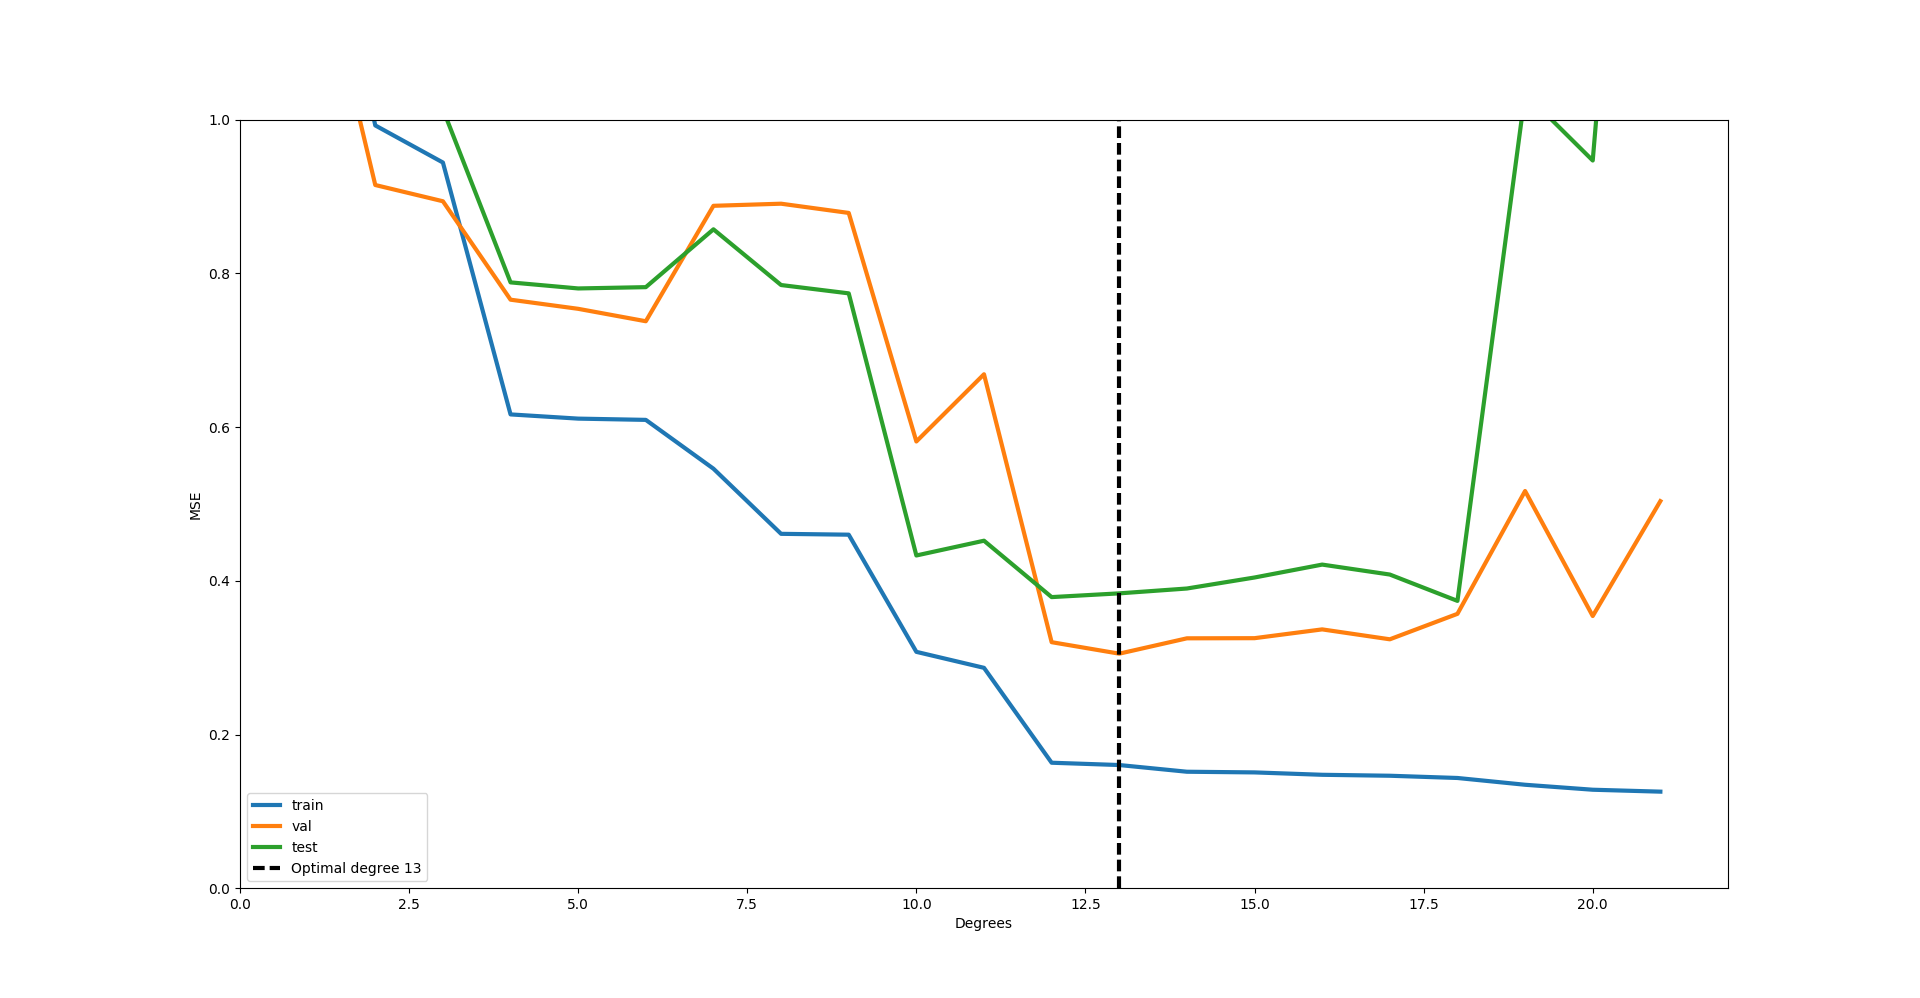
\includegraphics[width=\textwidth]{figures/linreg_errors.png}
	    \caption{Training, validation and testing errors}
	\end{figure}
	\begin{figure}[H]
	\centering
	        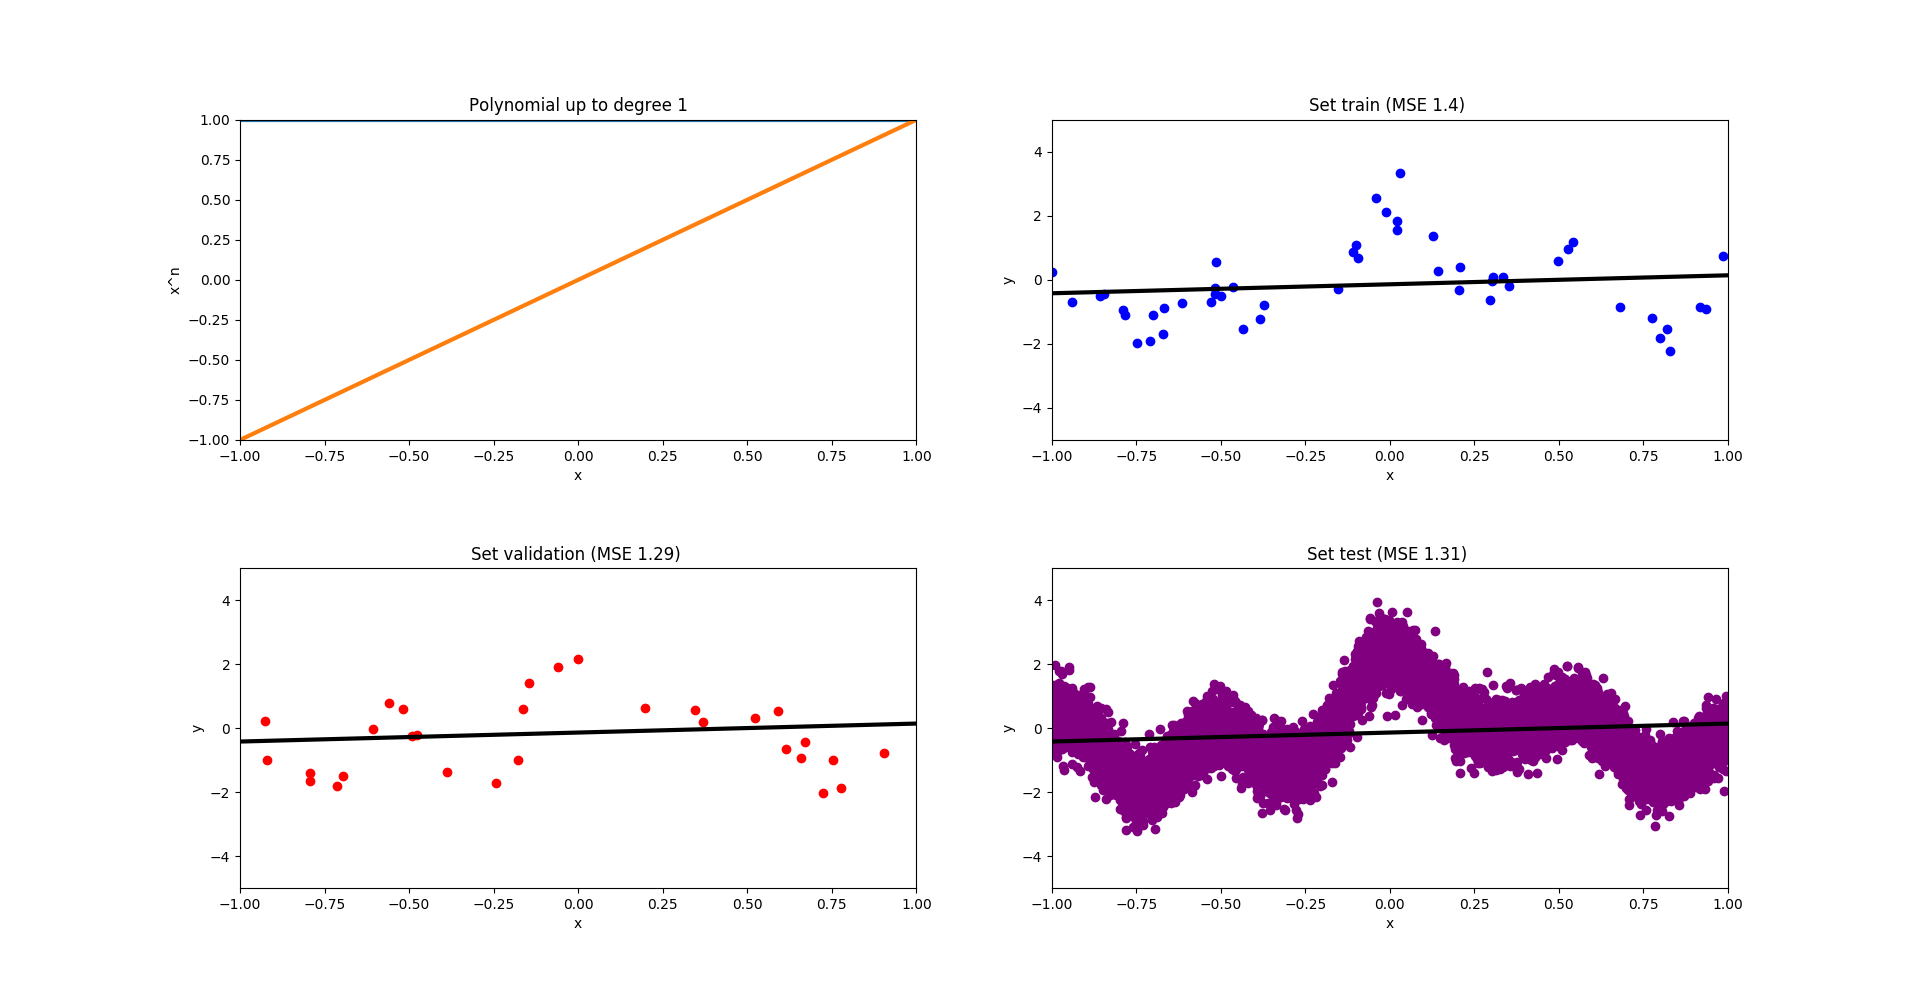
\includegraphics[width=\textwidth]{figures/linreg_degree_1.png}
	    \caption{Linear Regression (Polynomial, Degree 1)}
	\end{figure}
	\begin{figure}[H]
	\centering
	        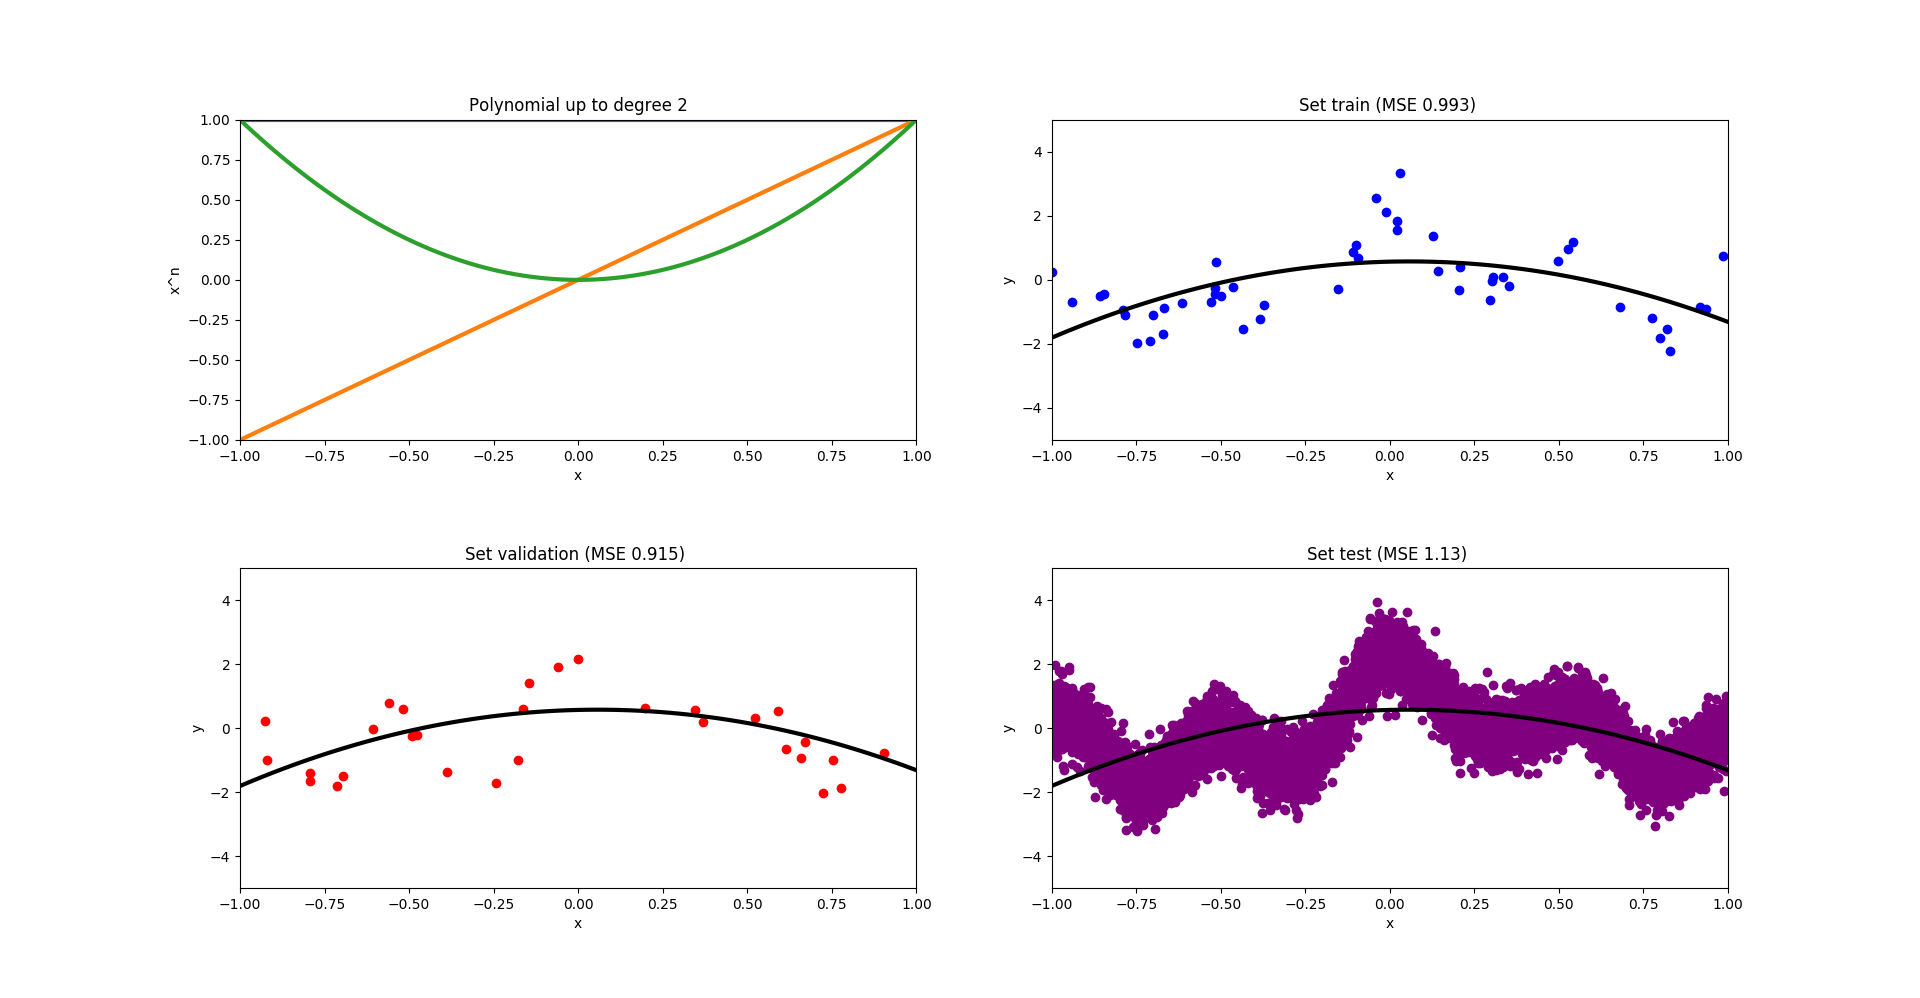
\includegraphics[width=\textwidth]{figures/linreg_degree_2.png}
	    \caption{Linear Regression (Polynomial, Degree 2)}
	\end{figure}
	\begin{figure}[H]
	\centering
	        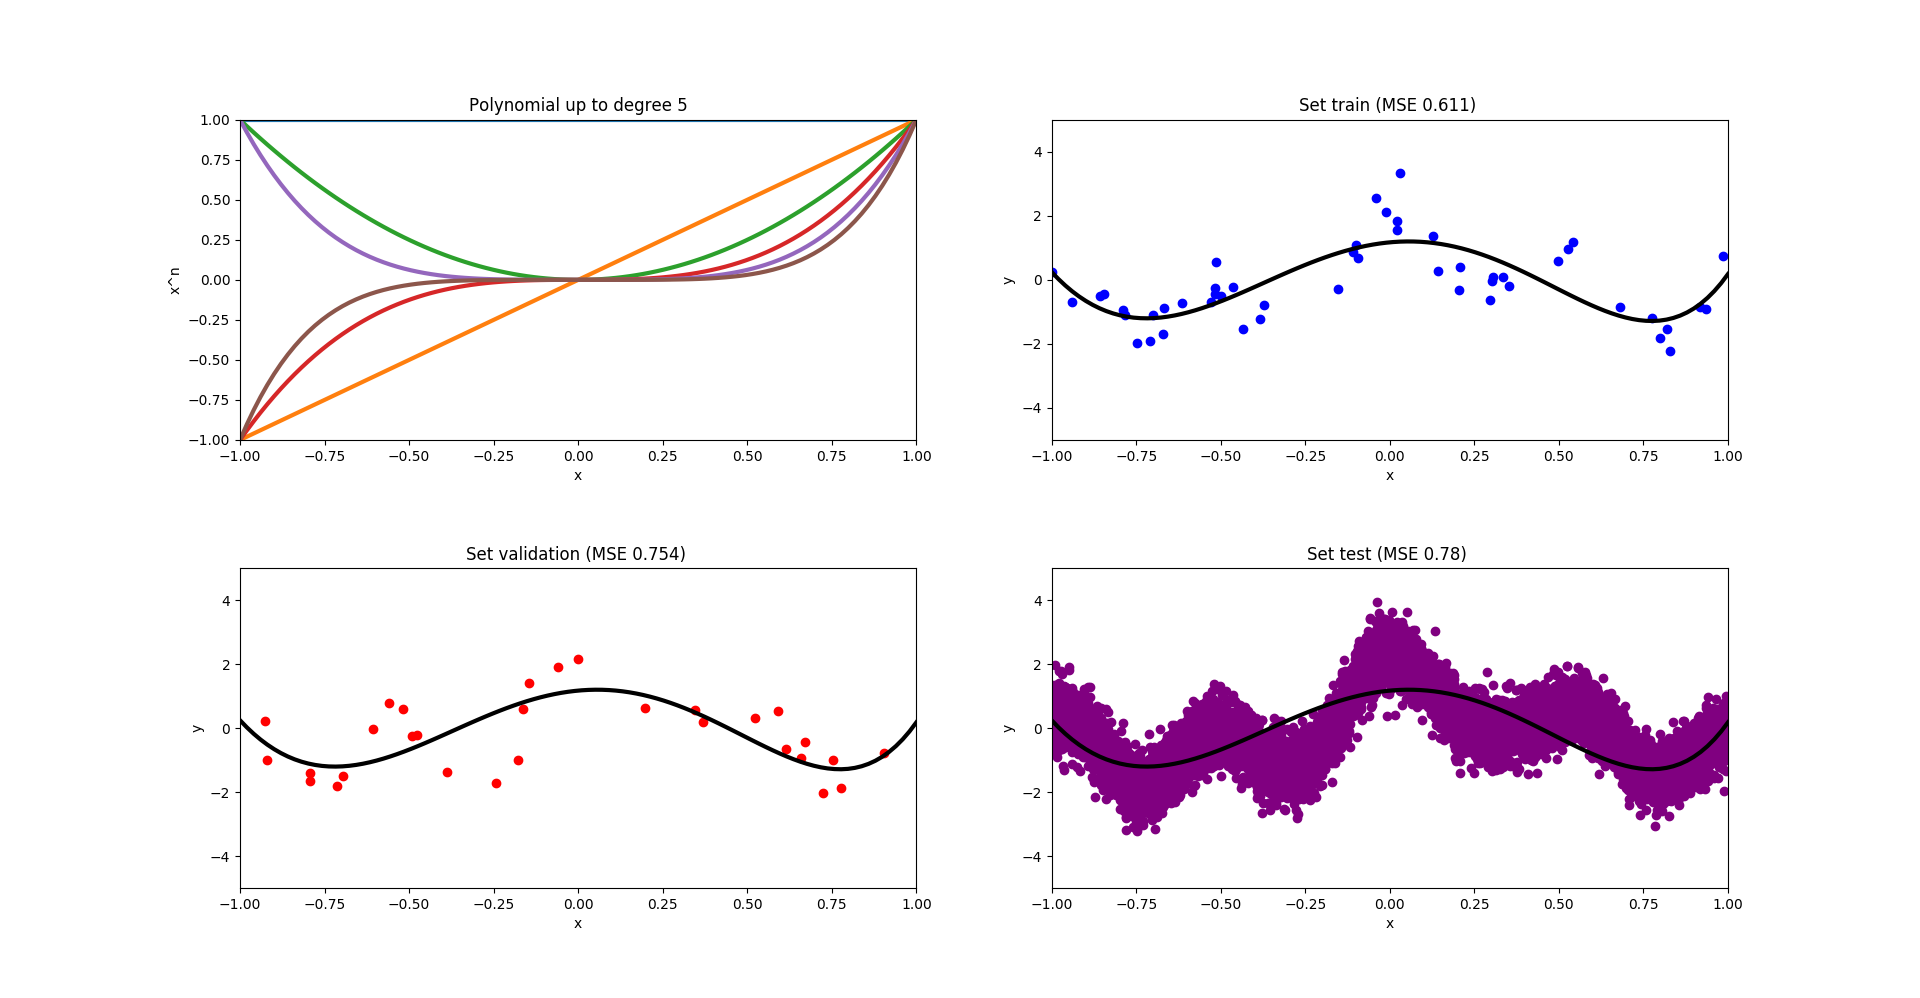
\includegraphics[width=\textwidth]{figures/linreg_degree_5.png}
	    \caption{Linear Regression (Polynomial, Degree 5)}
	\end{figure}
	\begin{figure}[H]
	\centering
	        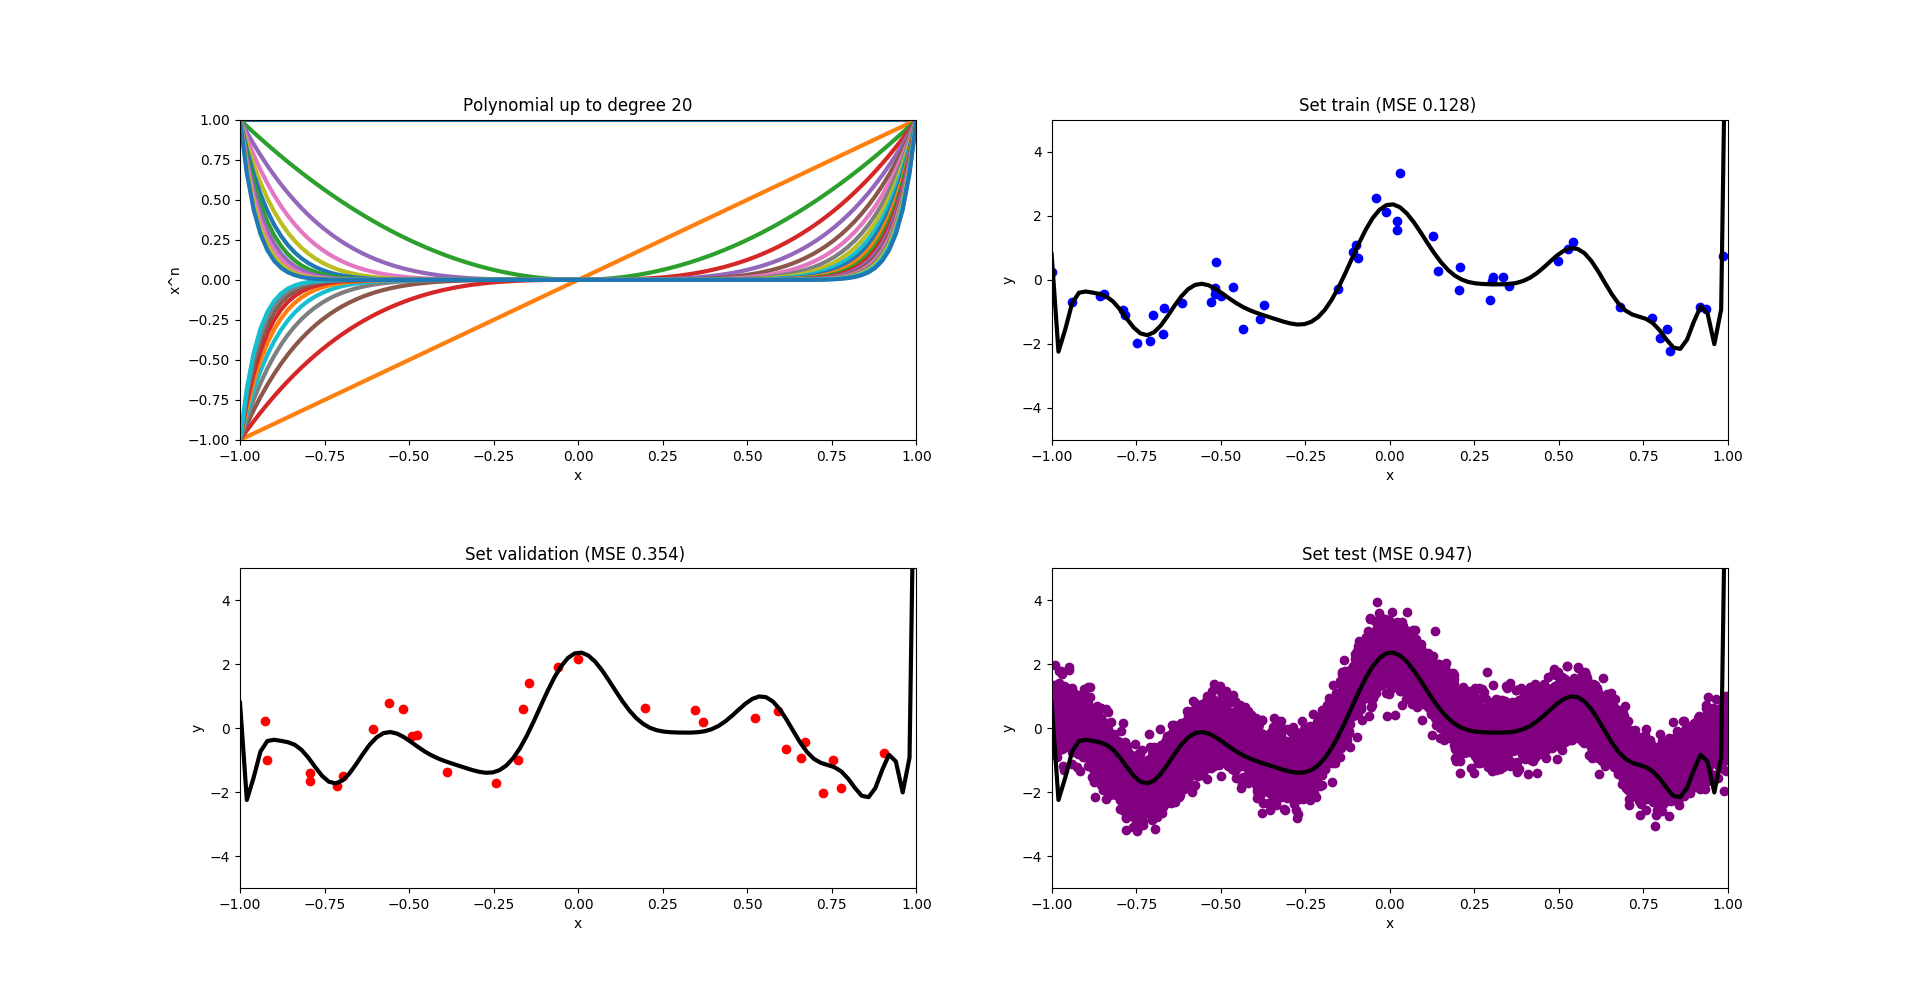
\includegraphics[width=\textwidth]{figures/linreg_degree_20.png}
	    \caption{Linear Regression (Polynomial, Degree 20)}
	\end{figure}
		
\begin{itemize}
  \item Lowest training error when using degree 21
  	\begin{figure}[H]
    \centering
	        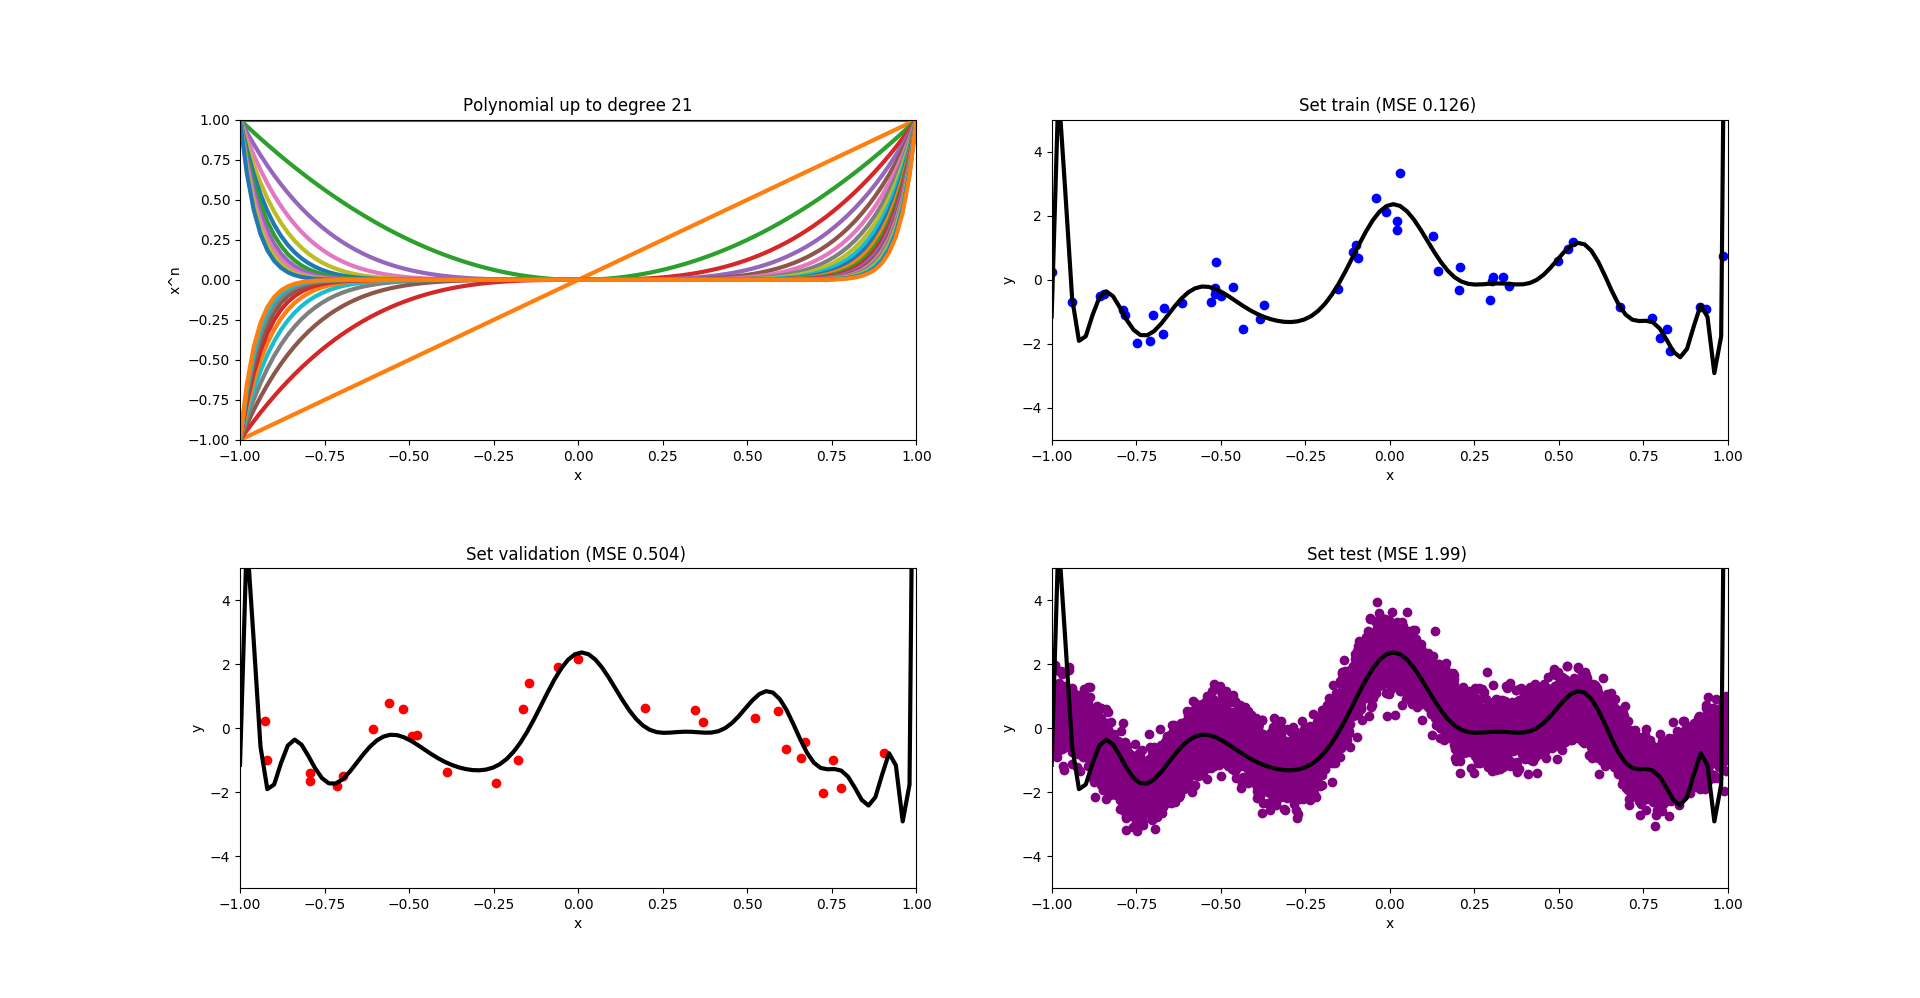
\includegraphics[width=\textwidth]{figures/linreg_degree_21.png}
	    \caption{Linear Regression (Polynomial, Degree 21)}
	\end{figure}
  \item Lowest validation error occurs when using degree 13
	\begin{figure}[H]
    \centering
	        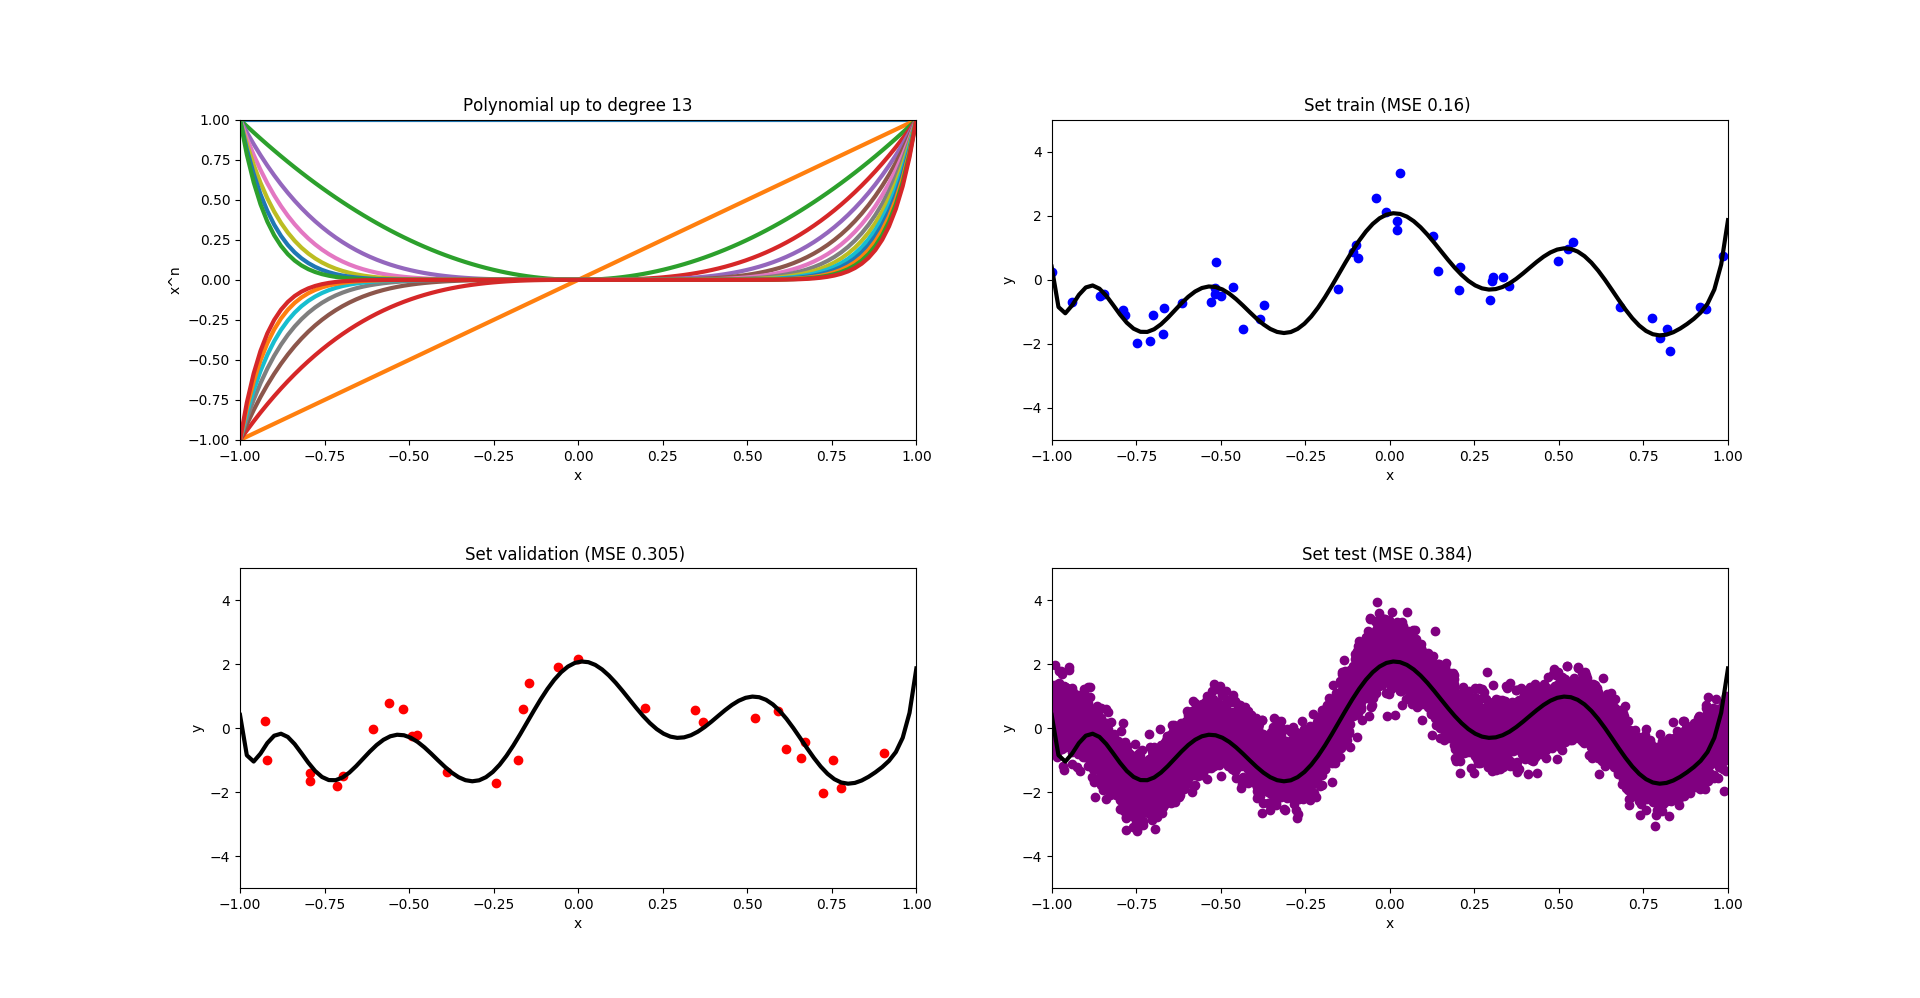
\includegraphics[width=\textwidth]{figures/linreg_degree_13.png}
	    \caption{Linear Regression (Polynomial, Degree 13)}
	\end{figure}
		
  \item \textbf{Discussion}\\
  Validation sets help to estimate performance of algorithms used for
  predictions and also to select a hypothesis (lowes error on set data).
  According to the error in the test set no over-fitting occured up to a
  degree of 13 (but would on higher degrees as can clearly be seen in Figure for
  degree 21, outliers and lesser data).
  
\end{itemize}
\subsection{Linear Regression with radial basis functions}
\begin{figure}[H]
	\centering
	        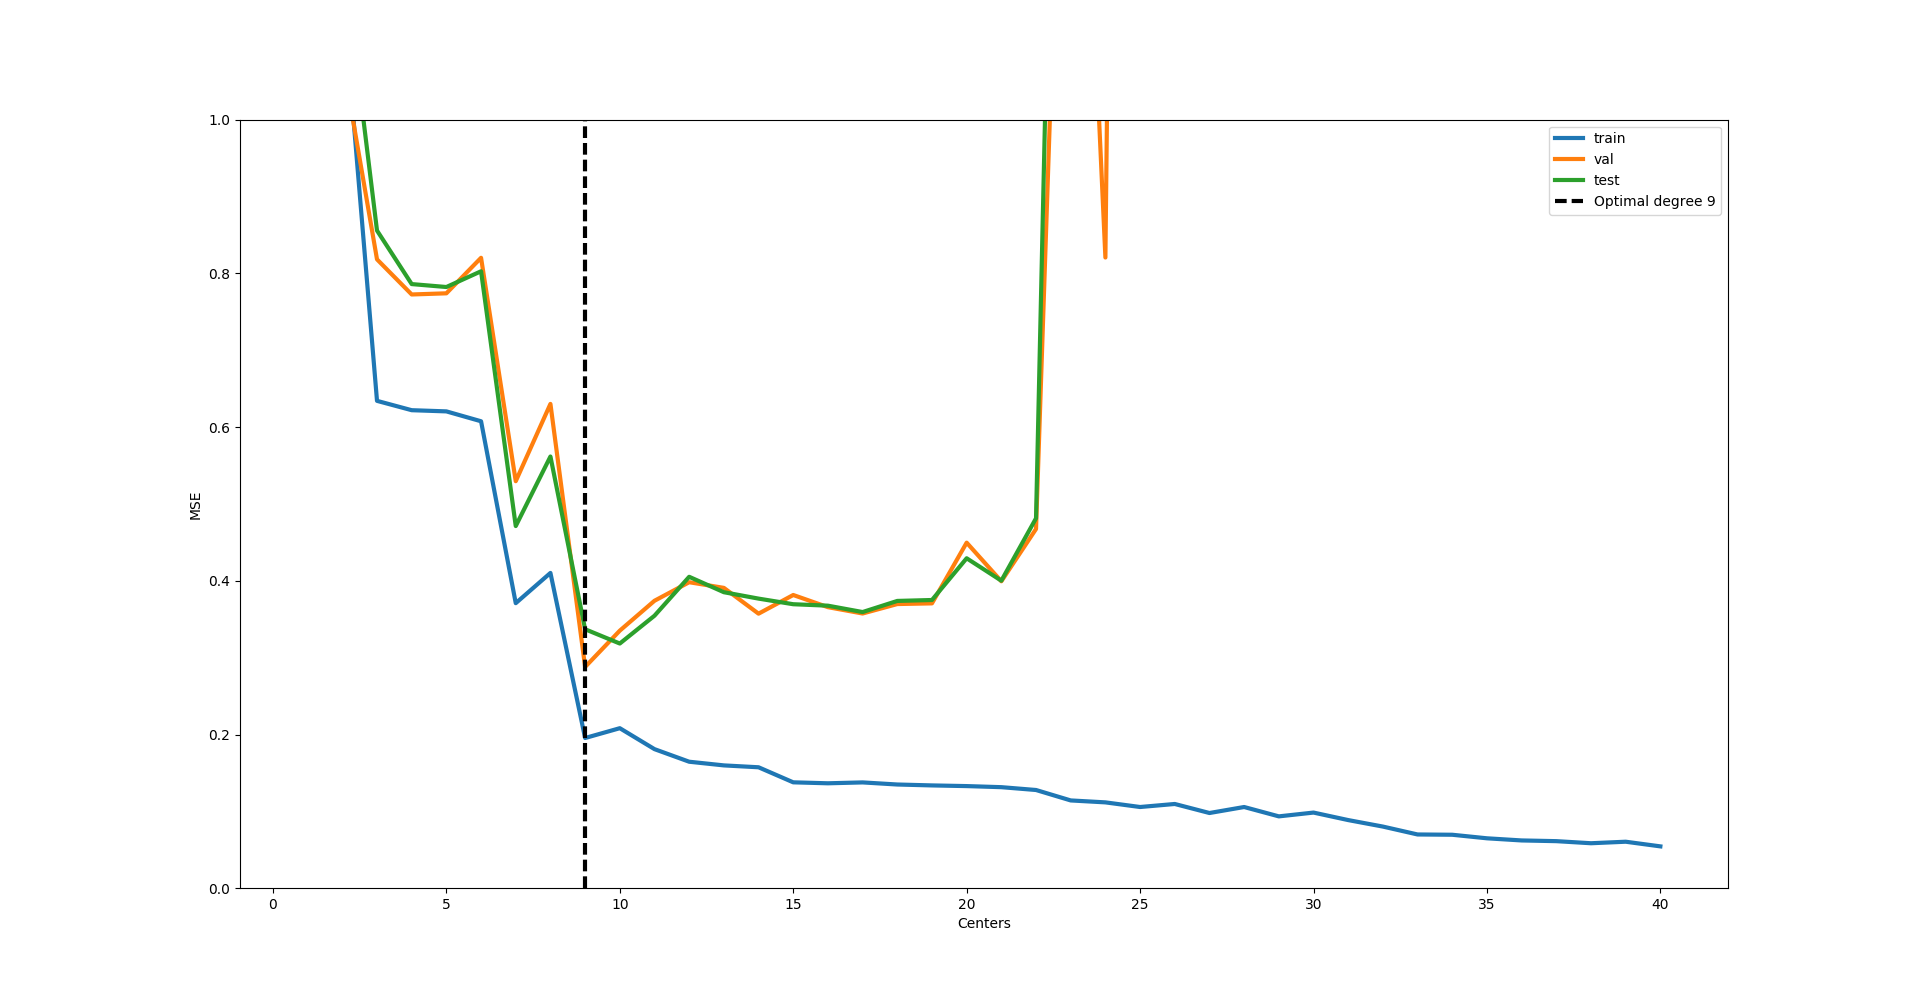
\includegraphics[width=\textwidth]{figures/linreg_bias_errors.png}
	    \caption{Training, validation and testing errors}
	\end{figure}
	\begin{figure}[H]
	\centering
	        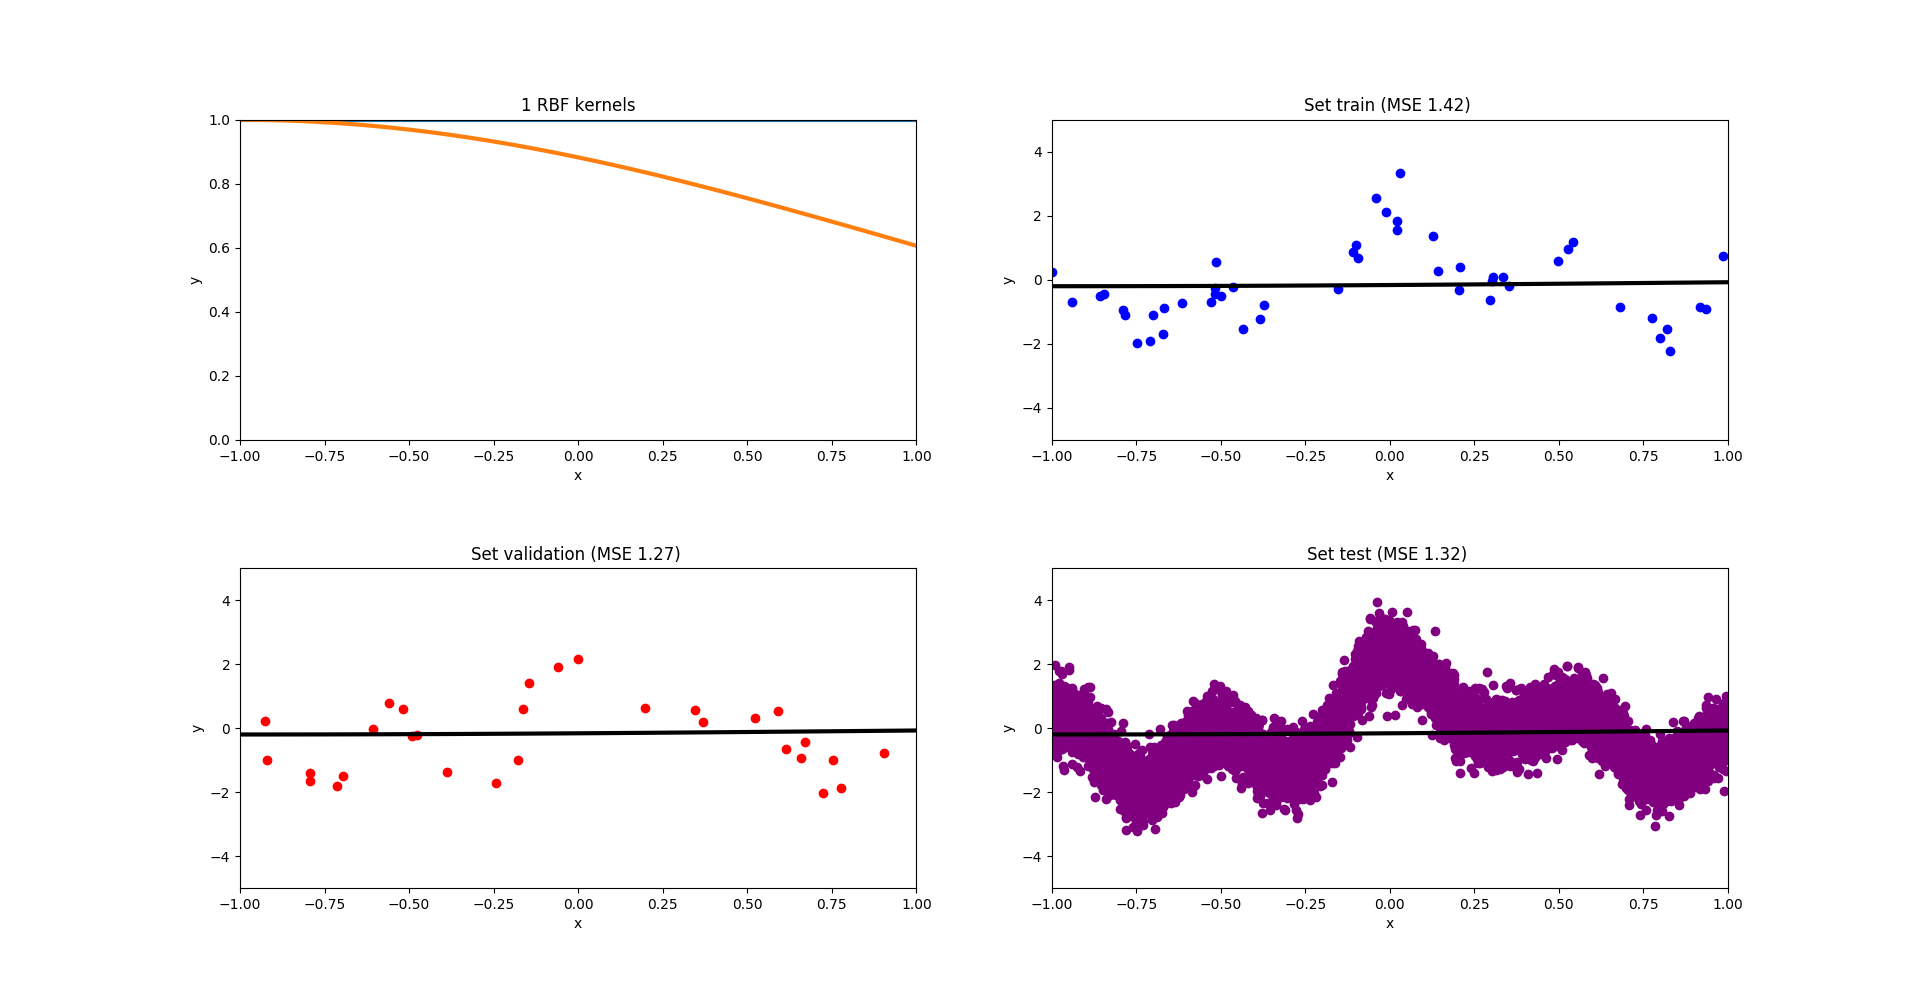
\includegraphics[width=\textwidth]{figures/linreg_bias_c1.png}
	    \caption{Linear Regression (Bias, Center 1)}
	\end{figure}
	\begin{figure}[H]
	\centering
	        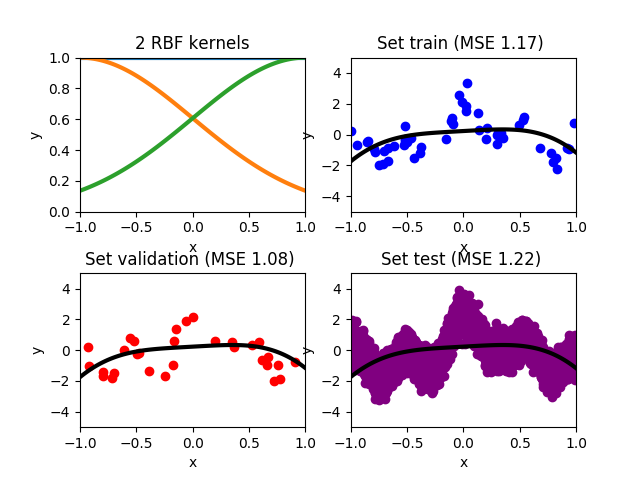
\includegraphics[width=\textwidth]{figures/linreg_bias_c2.png}
	    \caption{Linear Regression (Bias, Center 2)}
	\end{figure}
	\begin{figure}[H]
	\centering
	        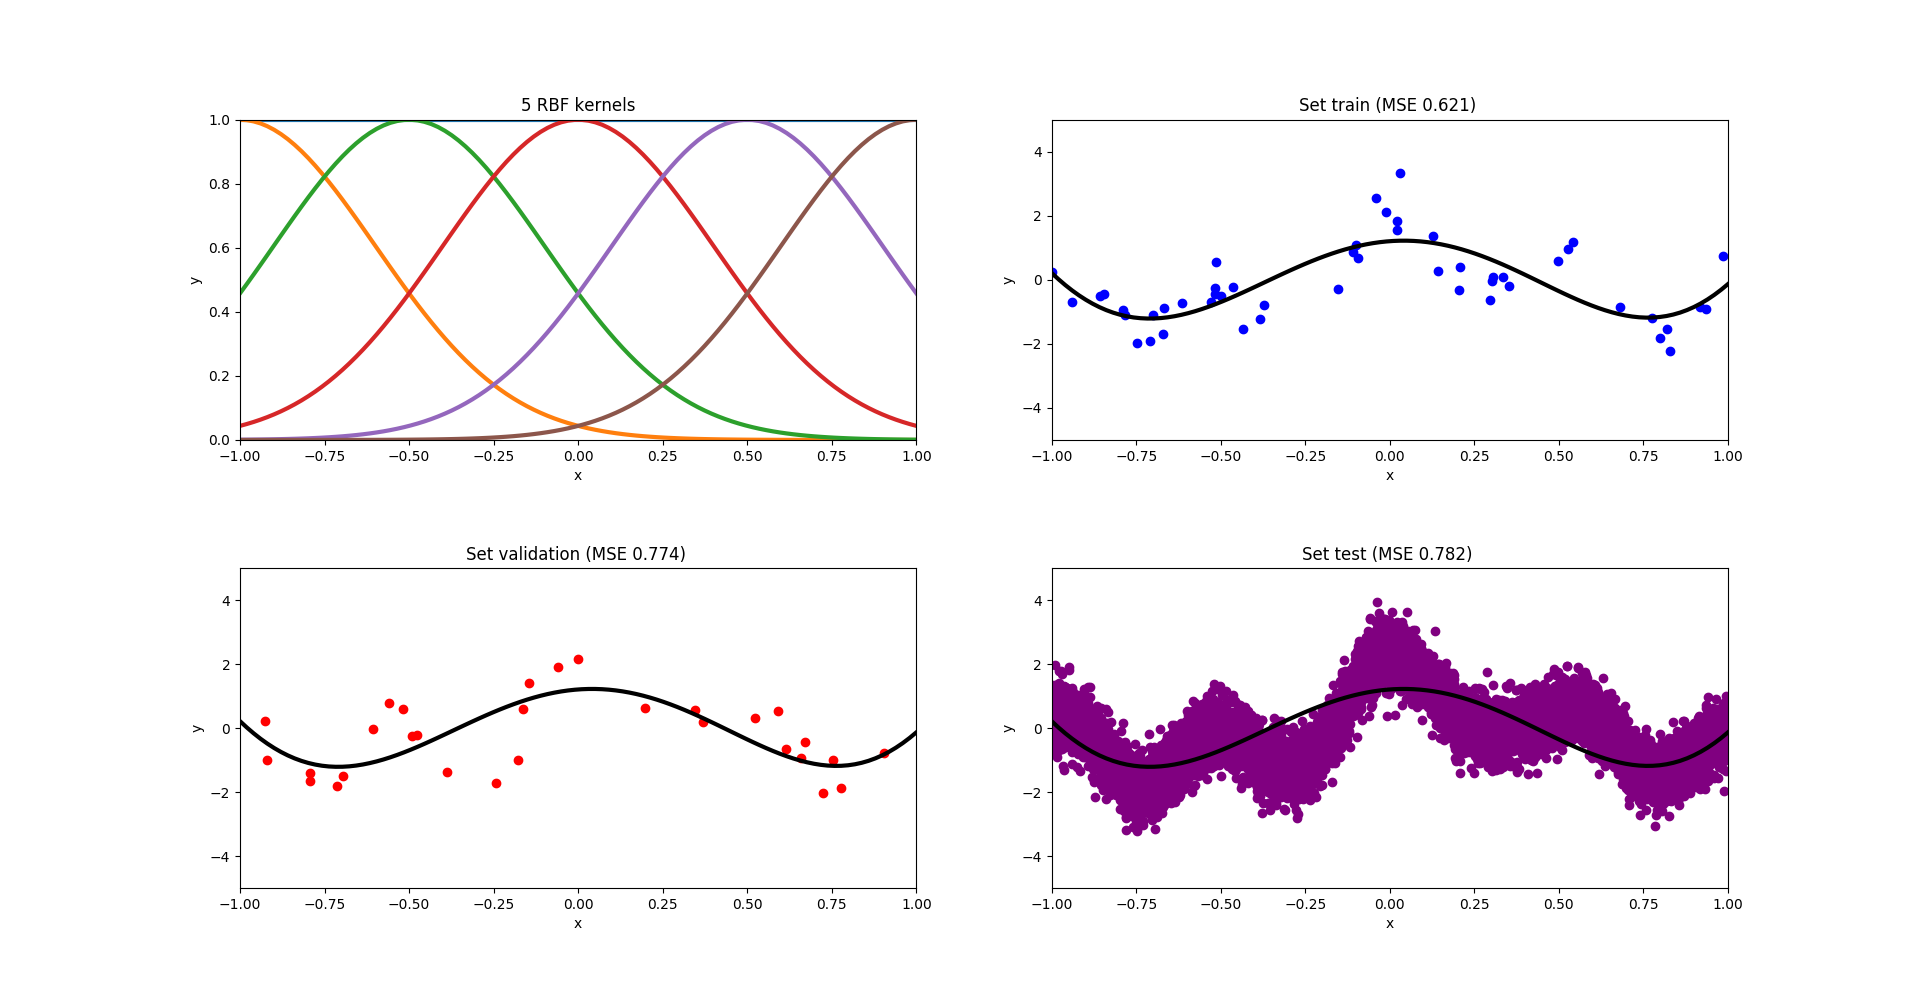
\includegraphics[width=\textwidth]{figures/linreg_bias_c5.png}
	    \caption{Linear Regression (Bias, Center 5)}
	\end{figure}
	\begin{figure}[H]
	\centering
	        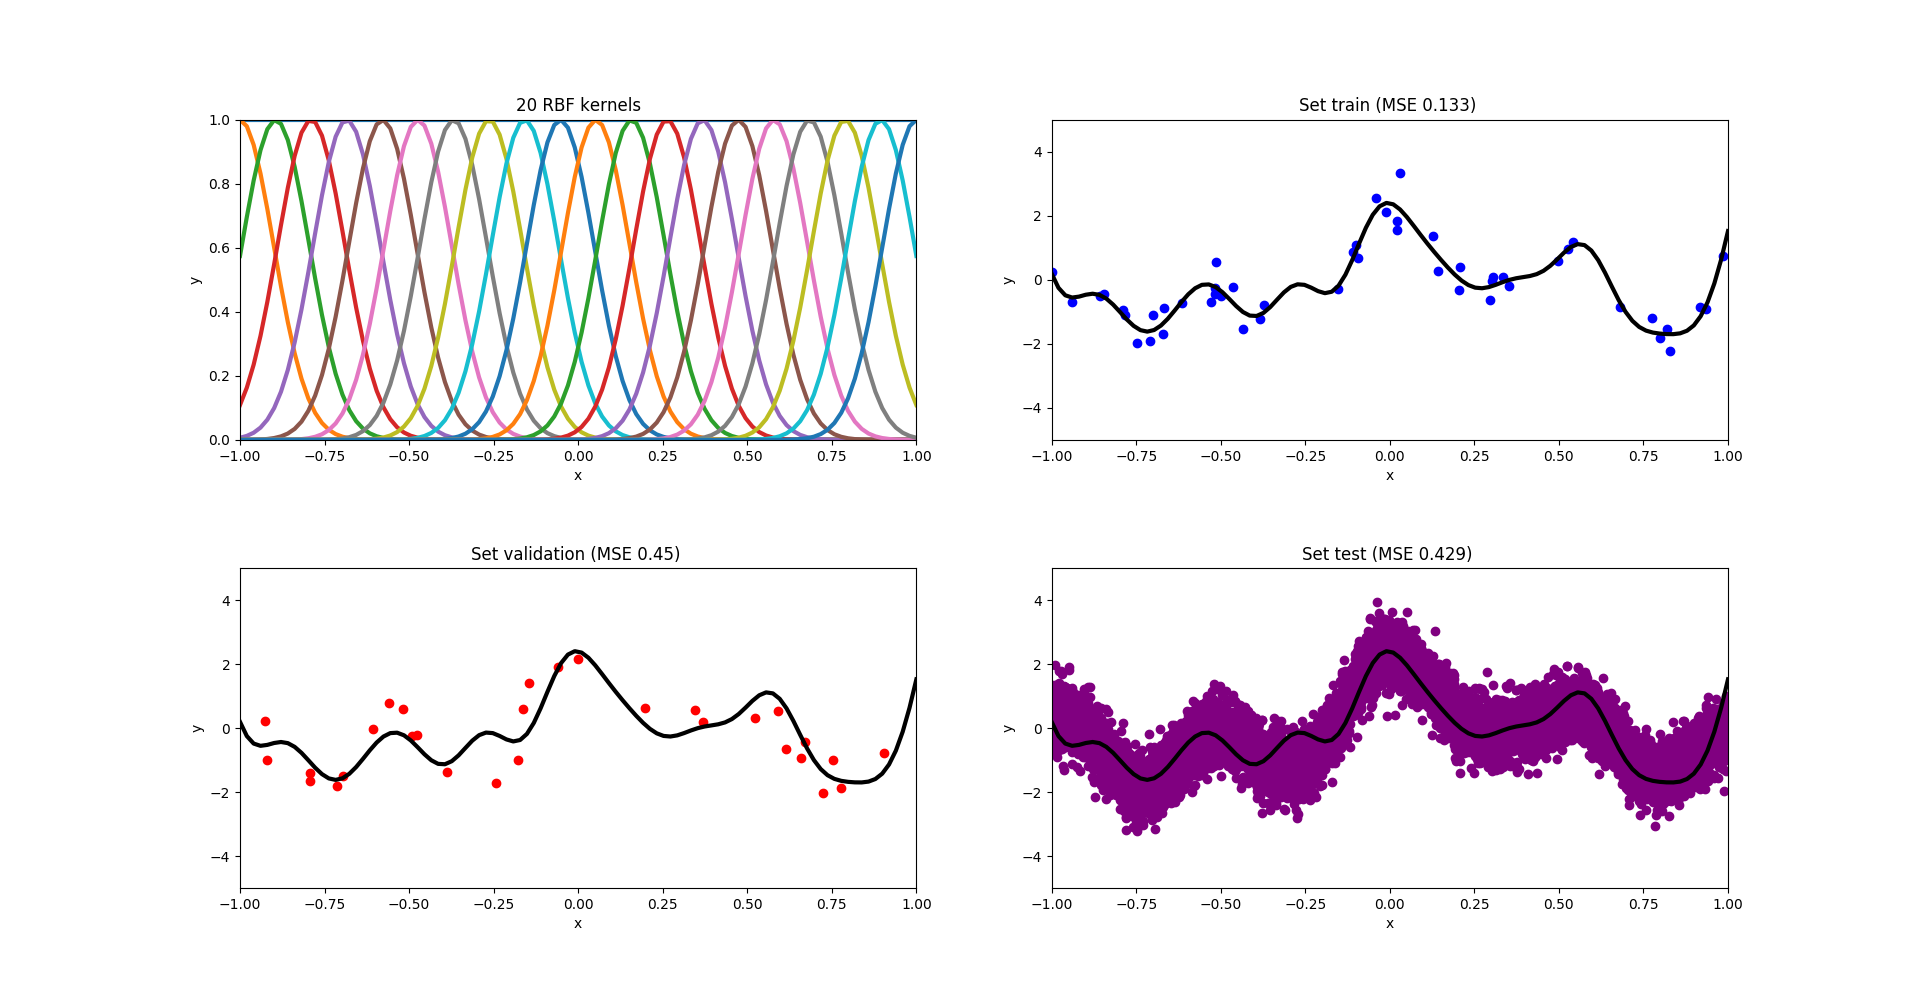
\includegraphics[width=\textwidth]{figures/linreg_bias_c20.png}
	    \caption{Linear Regression (Bias, Center 20)}
	\end{figure}
\begin{itemize}
  \item Lowest training error when using center 40
  	\begin{figure}[H]
    \centering
	        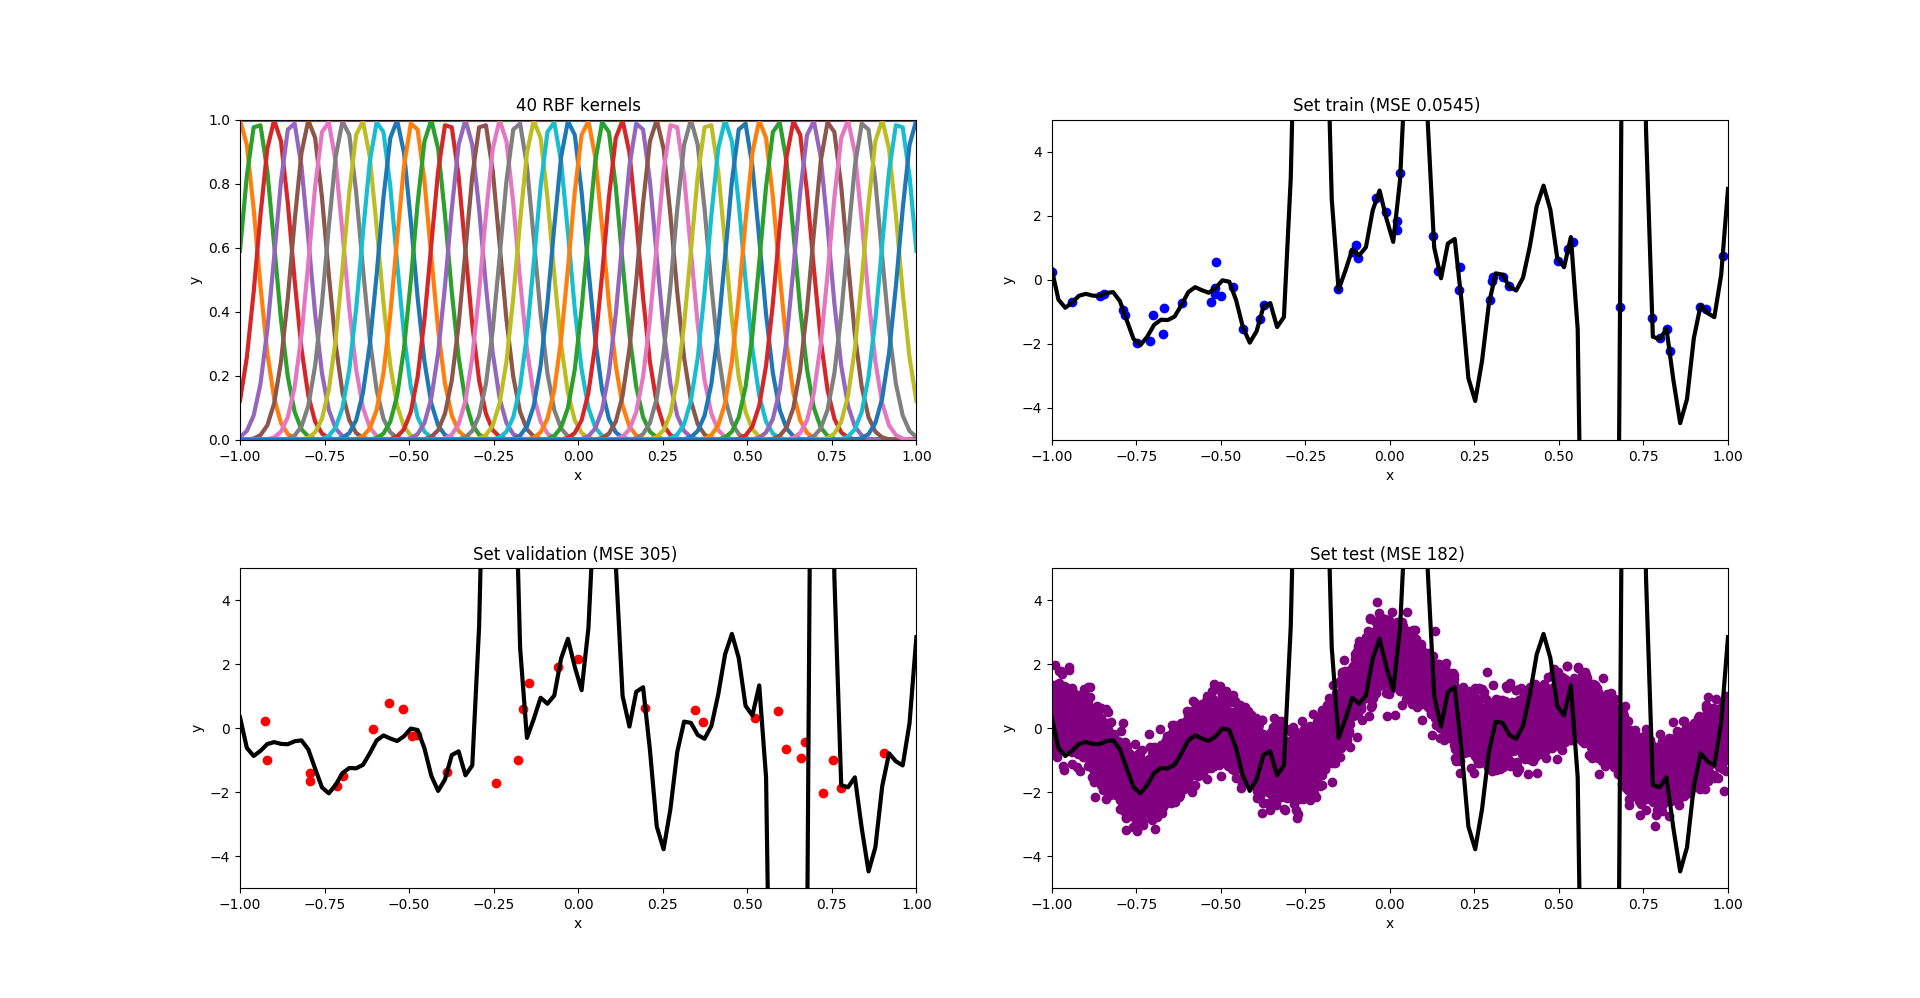
\includegraphics[width=\textwidth]{figures/linreg_bias_c40.png}
	    \caption{Linear Regression (Bias, Center 40)}
	\end{figure}
  \item Lowest validation error occurs when using center 9
	\begin{figure}[H]
    \centering
	        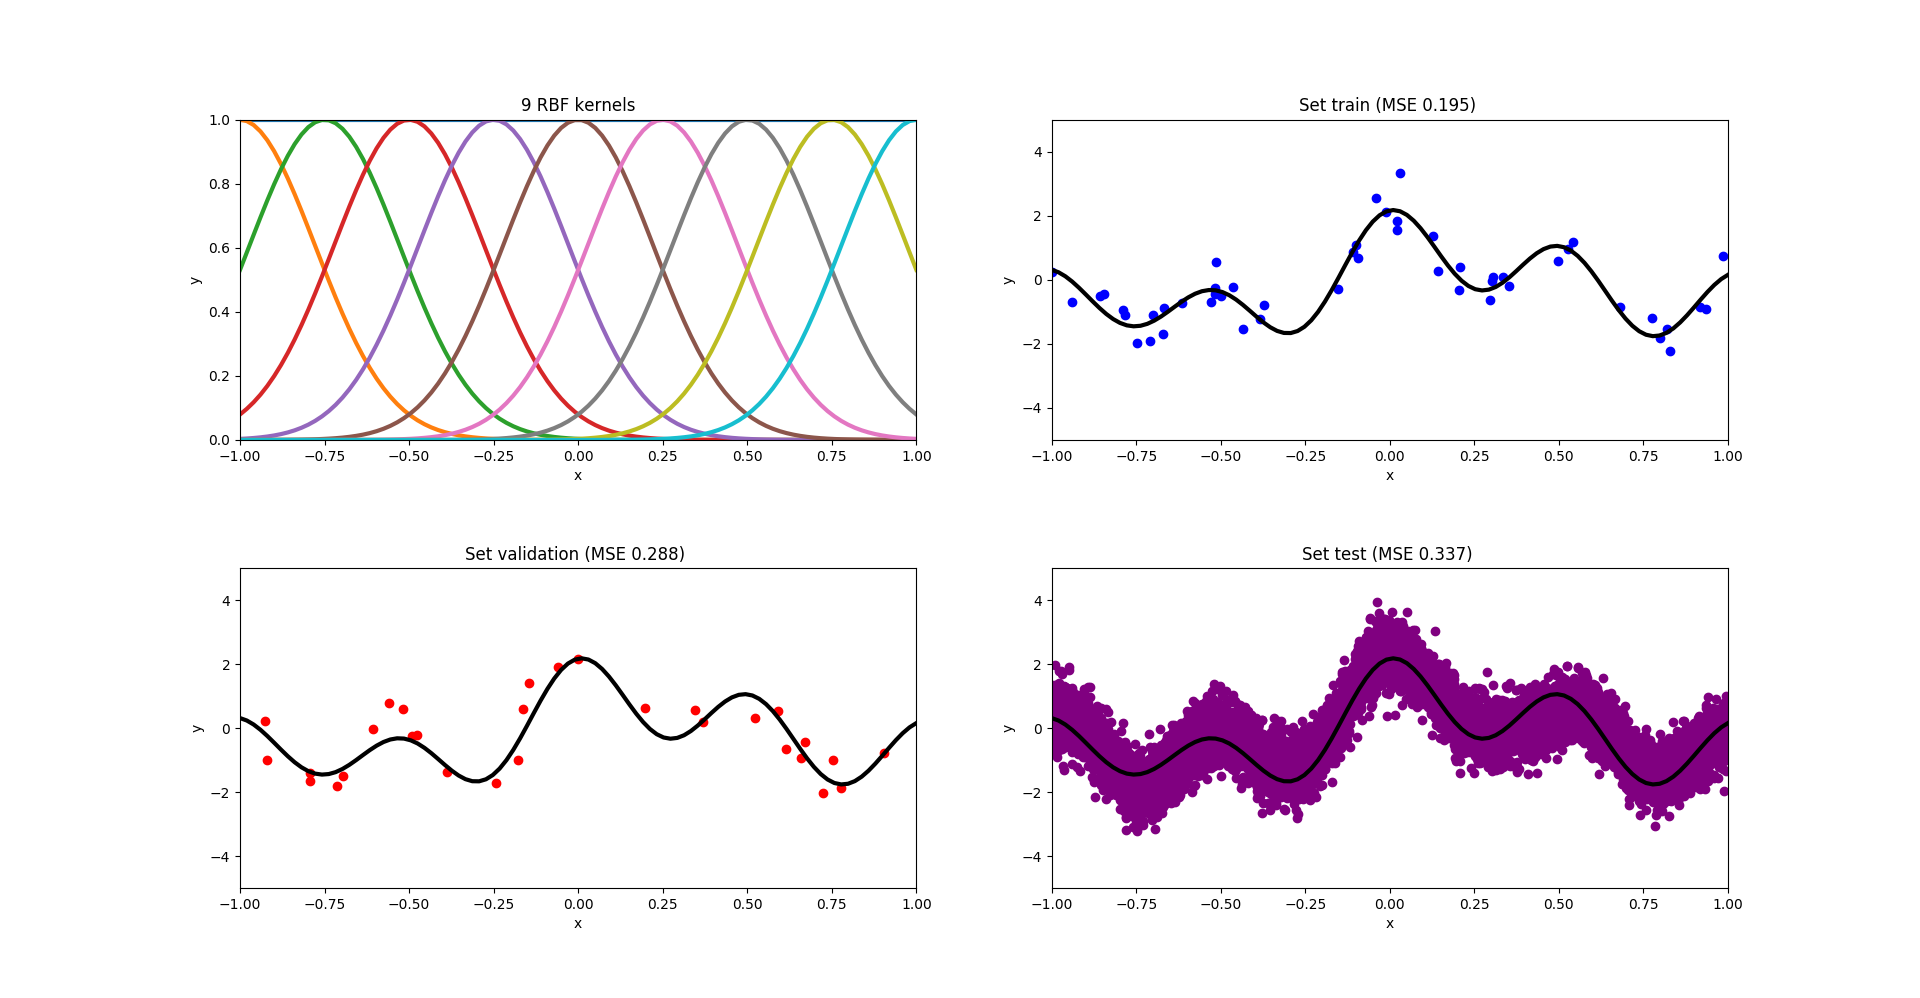
\includegraphics[width=\textwidth]{figures/linreg_bias_c9.png}
	    \caption{Linear Regression (Polynomial, Degree 9)}
	\end{figure}
		
  \item \textbf{Discussion}\\
  Bias function is better because it fits natural phenomen better. Overfitting
  occurs very early on parameter center 10.
  
\end{itemize}

\section{Logistic Regression}

\subsection{Derivation of Gradient}

\subsection{Logistic Regression training with gradient descent and scipy.optimize}

\subsubsection{Gradient descent}
\begin{enumerate}
  \item \textbf{check\_gradient} explaination
  
  The function check whether the regression functions are really converging at a
  certain rate. To avoid divergence ;)
  \item \textbf{gradient descent} degree $l = 1$, 20 and 2000 iterations,
  learning rate $\eta = 1$
  	\begin{figure}[H]
  	\centering
	        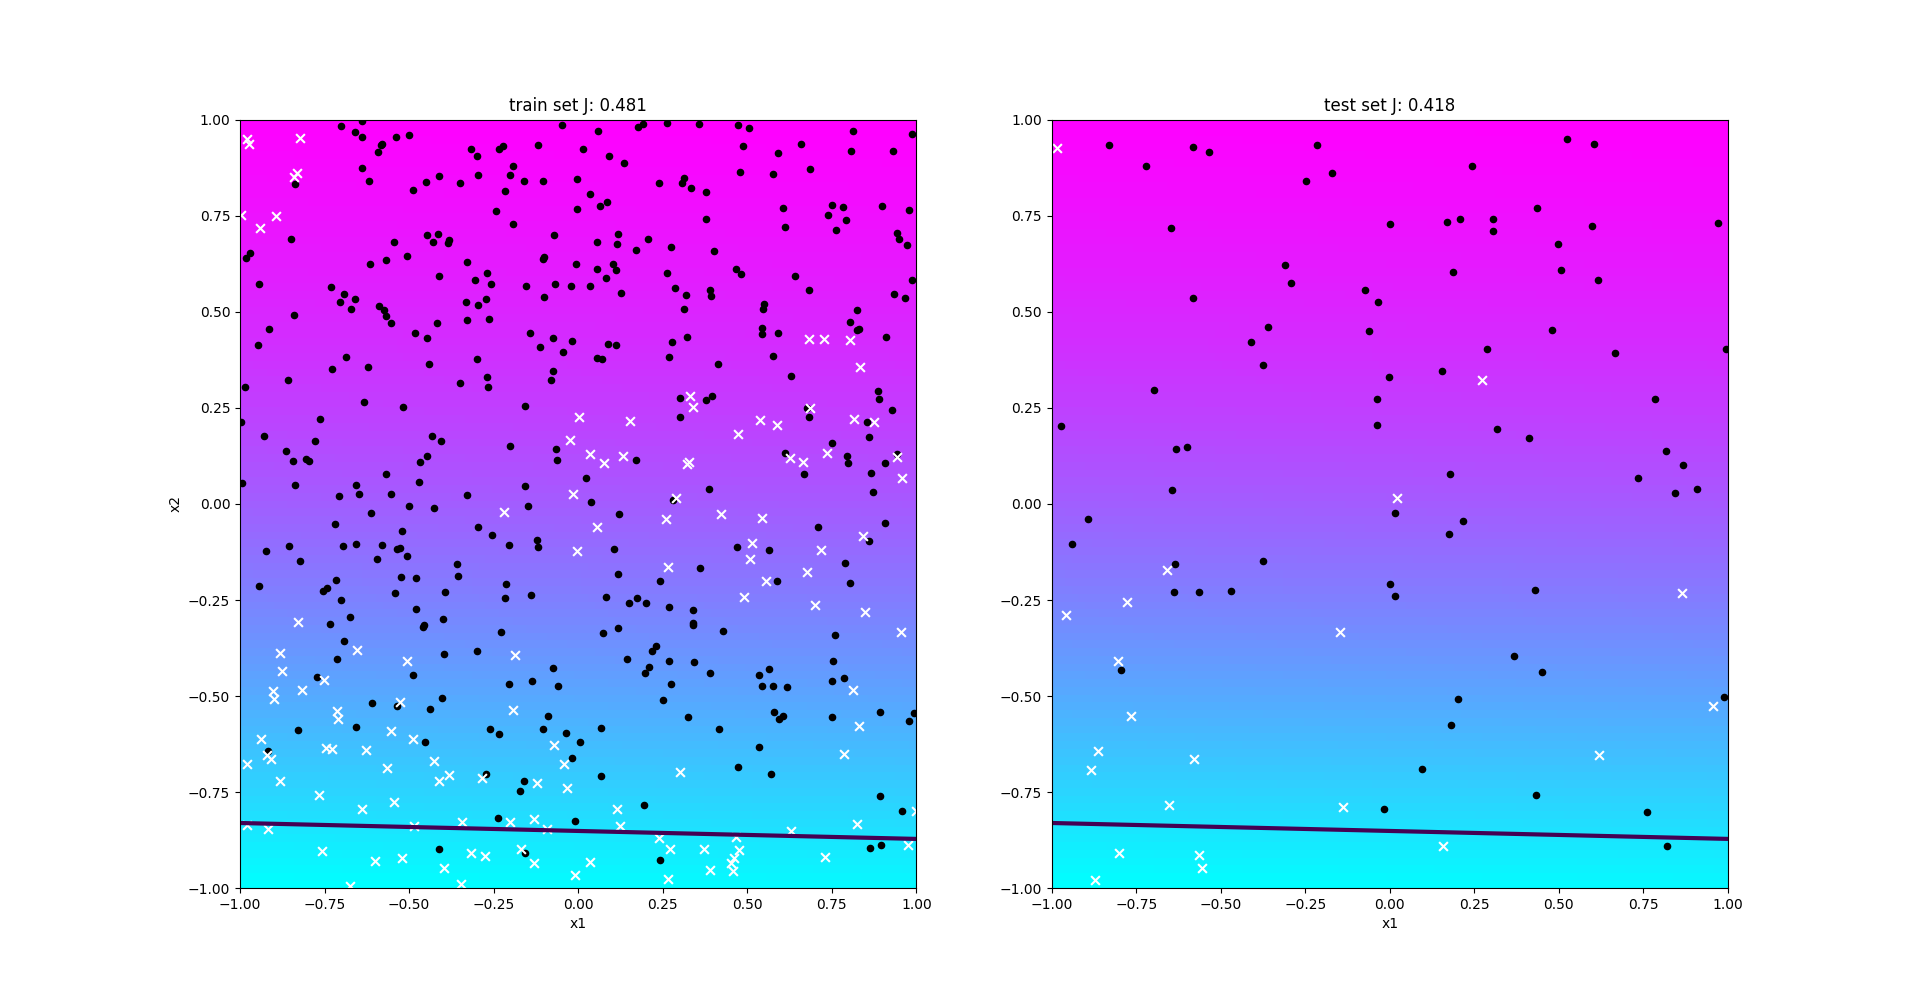
\includegraphics[width=\textwidth]{figures/logreg_d5_it20_1.png}
	    \caption{Logistic Regression ($\eta = 1$, $l = 1$, 20 iterations)}
	\end{figure}
	\begin{figure}[H]
  	\centering
	        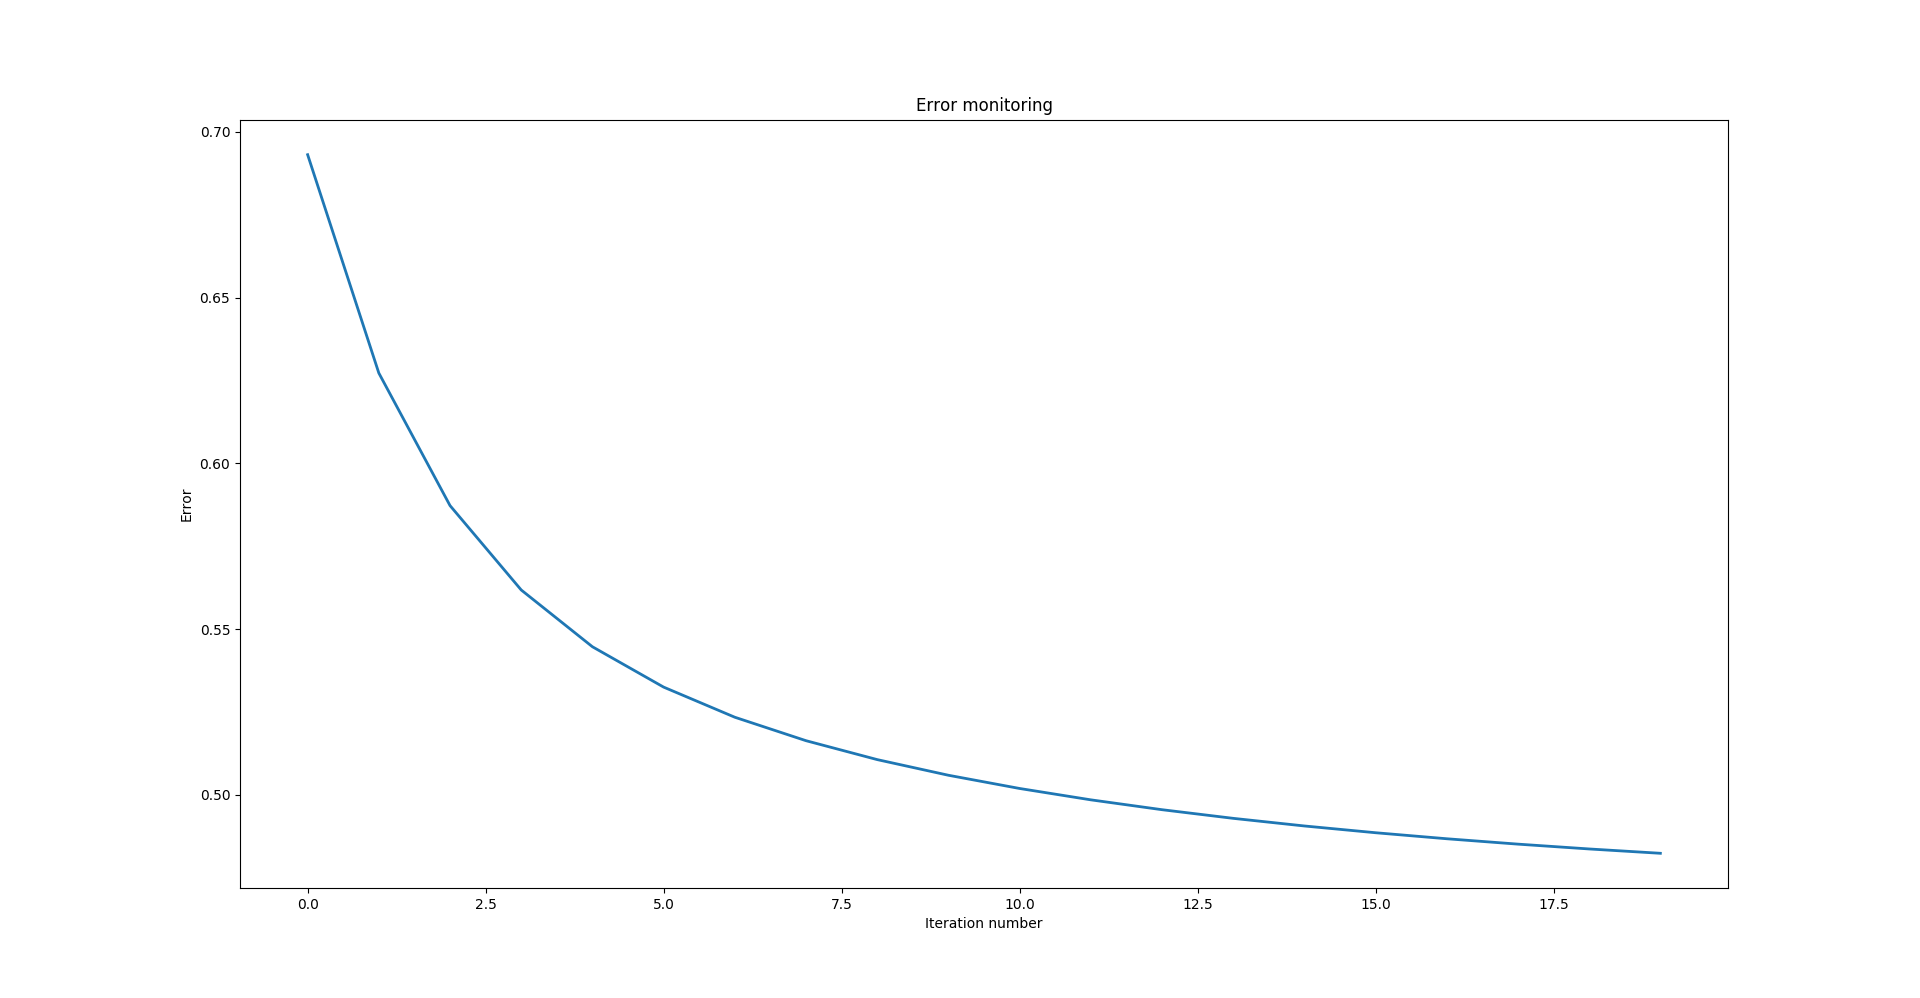
\includegraphics[width=\textwidth]{figures/logreg_d5_it20_1_error.png}
	    \caption{Logistic Regression Errors ($\eta = 1$, $l = 1$, 20 iterations)}
	\end{figure}
	\begin{figure}[H]
  	\centering
	        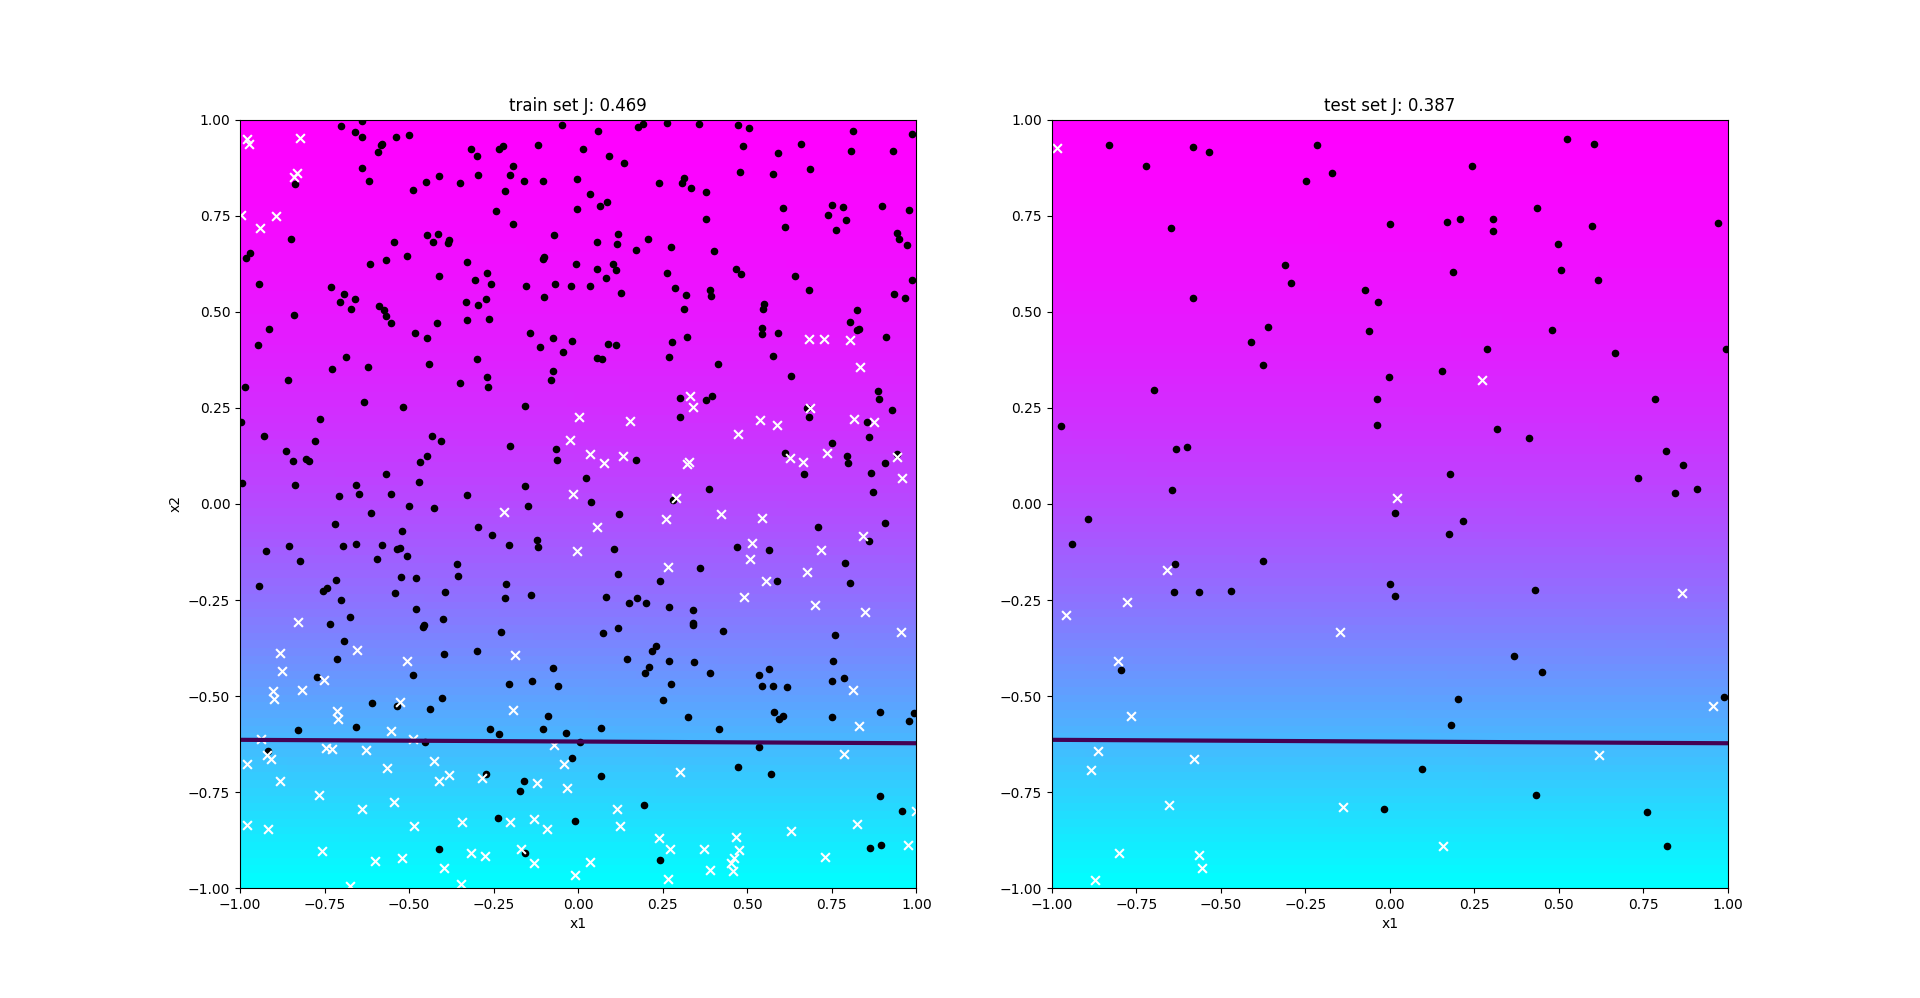
\includegraphics[width=\textwidth]{figures/logreg_d5_it2000_1.png}
	    \caption{Logistic Regression ($\eta = 1$, $l = 1$, 2000 iterations)}
	\end{figure}
	\begin{figure}[H]
  	\centering
	        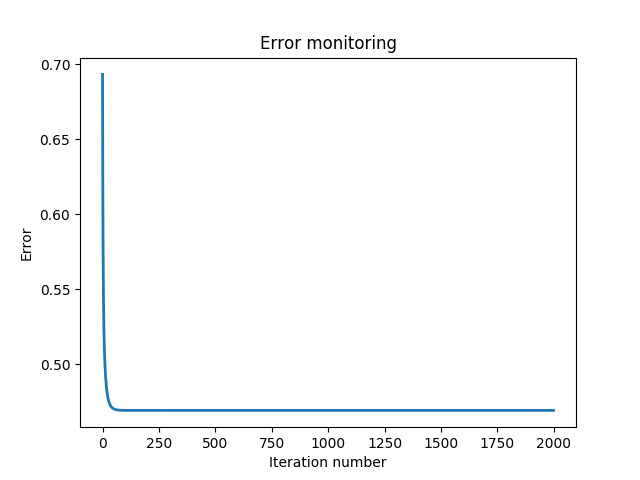
\includegraphics[width=\textwidth]{figures/logreg_d5_it2000_1_error.png}
	    \caption{Logistic Regression Errors ($\eta = 1$, $l = 1$, 2000 iterations)}
	\end{figure}
	\item \textbf{gradient descent} degree $l = 2$, 200 iterations,
	learning rate $\eta = 0.15, 1.5, 15$
	\begin{figure}[H]
  	\centering
	        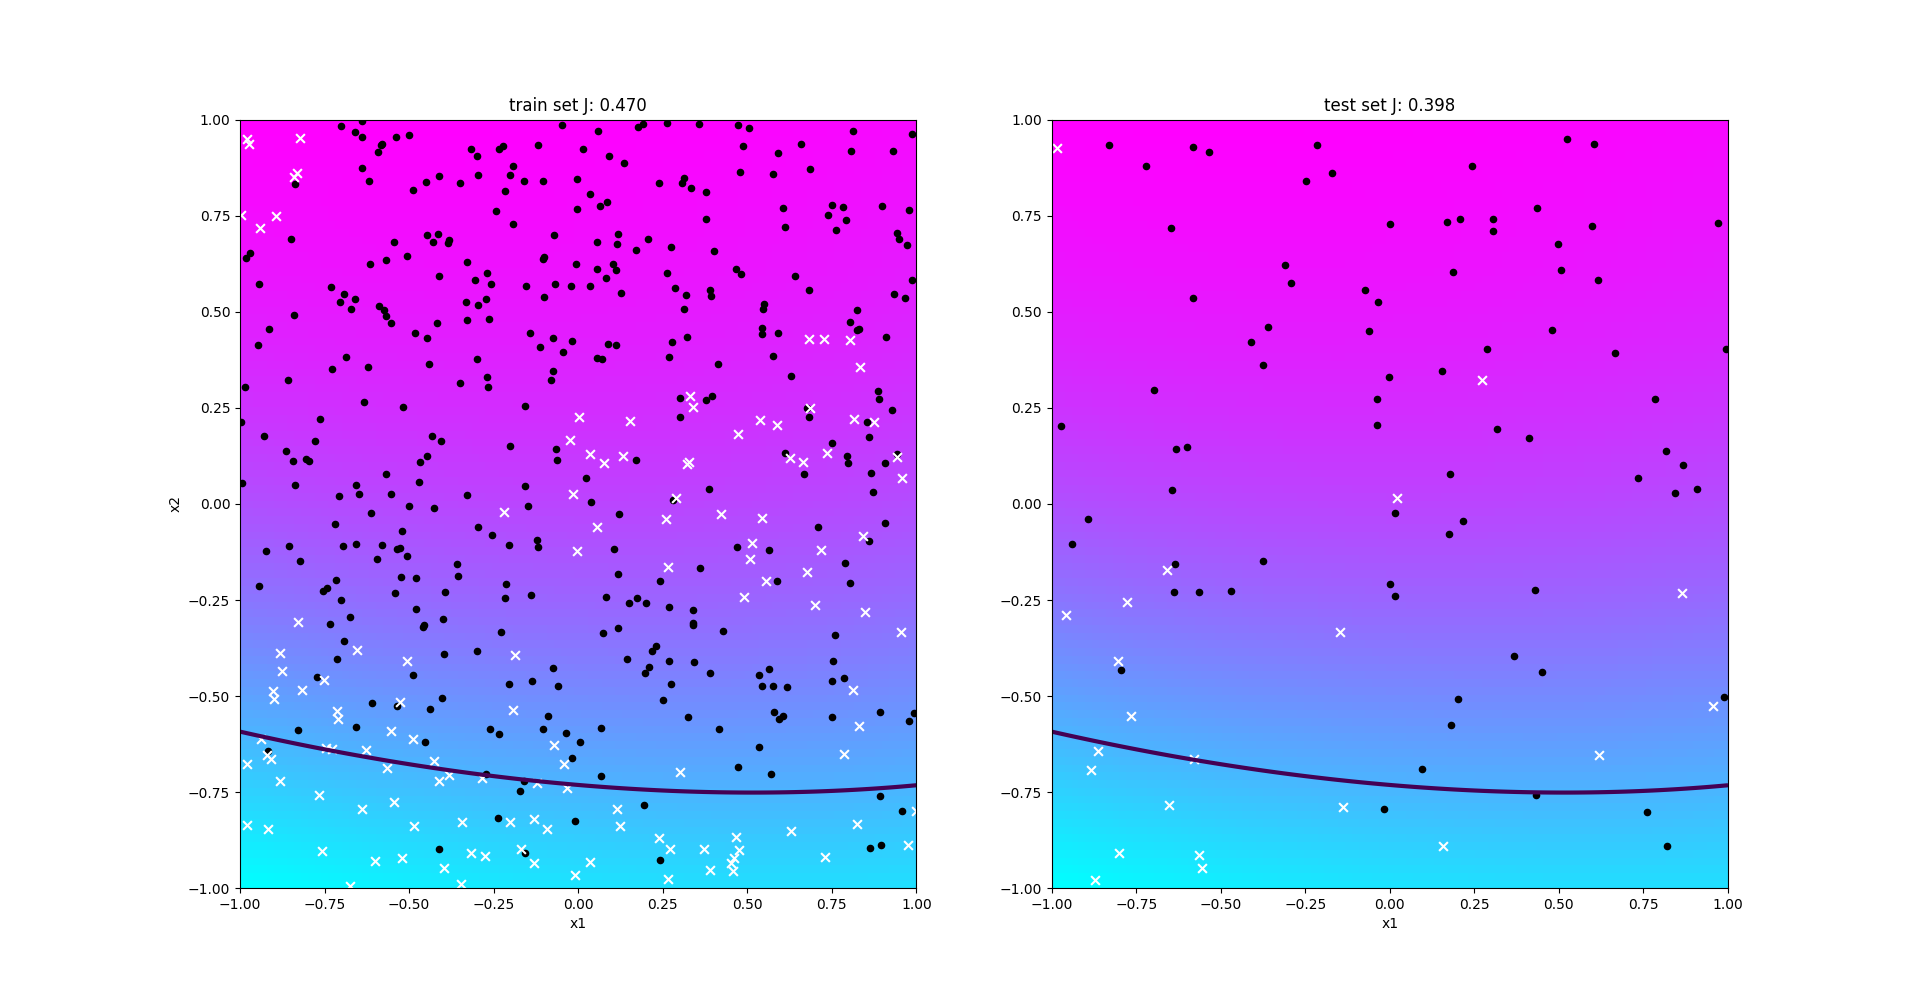
\includegraphics[width=\textwidth]{figures/logreg_d2_it200_015.png}
	    \caption{Logistic Regression ($\eta = 0.15$, $l = 1$, 200 iterations)}
	\end{figure}
	\begin{figure}[H]
  	\centering
	        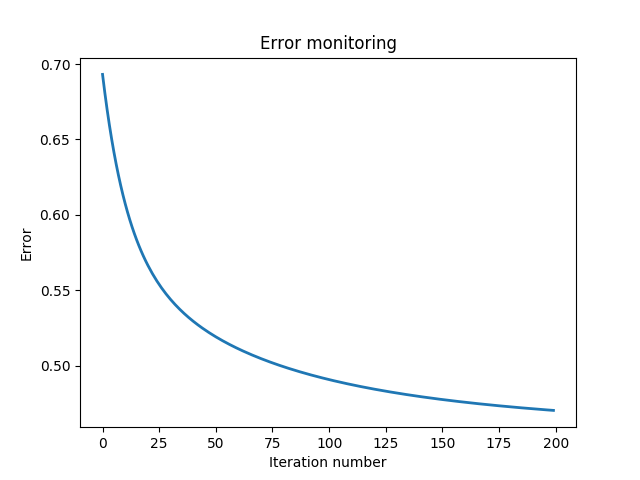
\includegraphics[width=\textwidth]{figures/logreg_d2_it200_015_error.png}
	    \caption{Logistic Regression Errors ($\eta = 0.15$, $l = 1$, 200
	    iterations)}
	\end{figure}
	\begin{figure}[H]
  	\centering
	        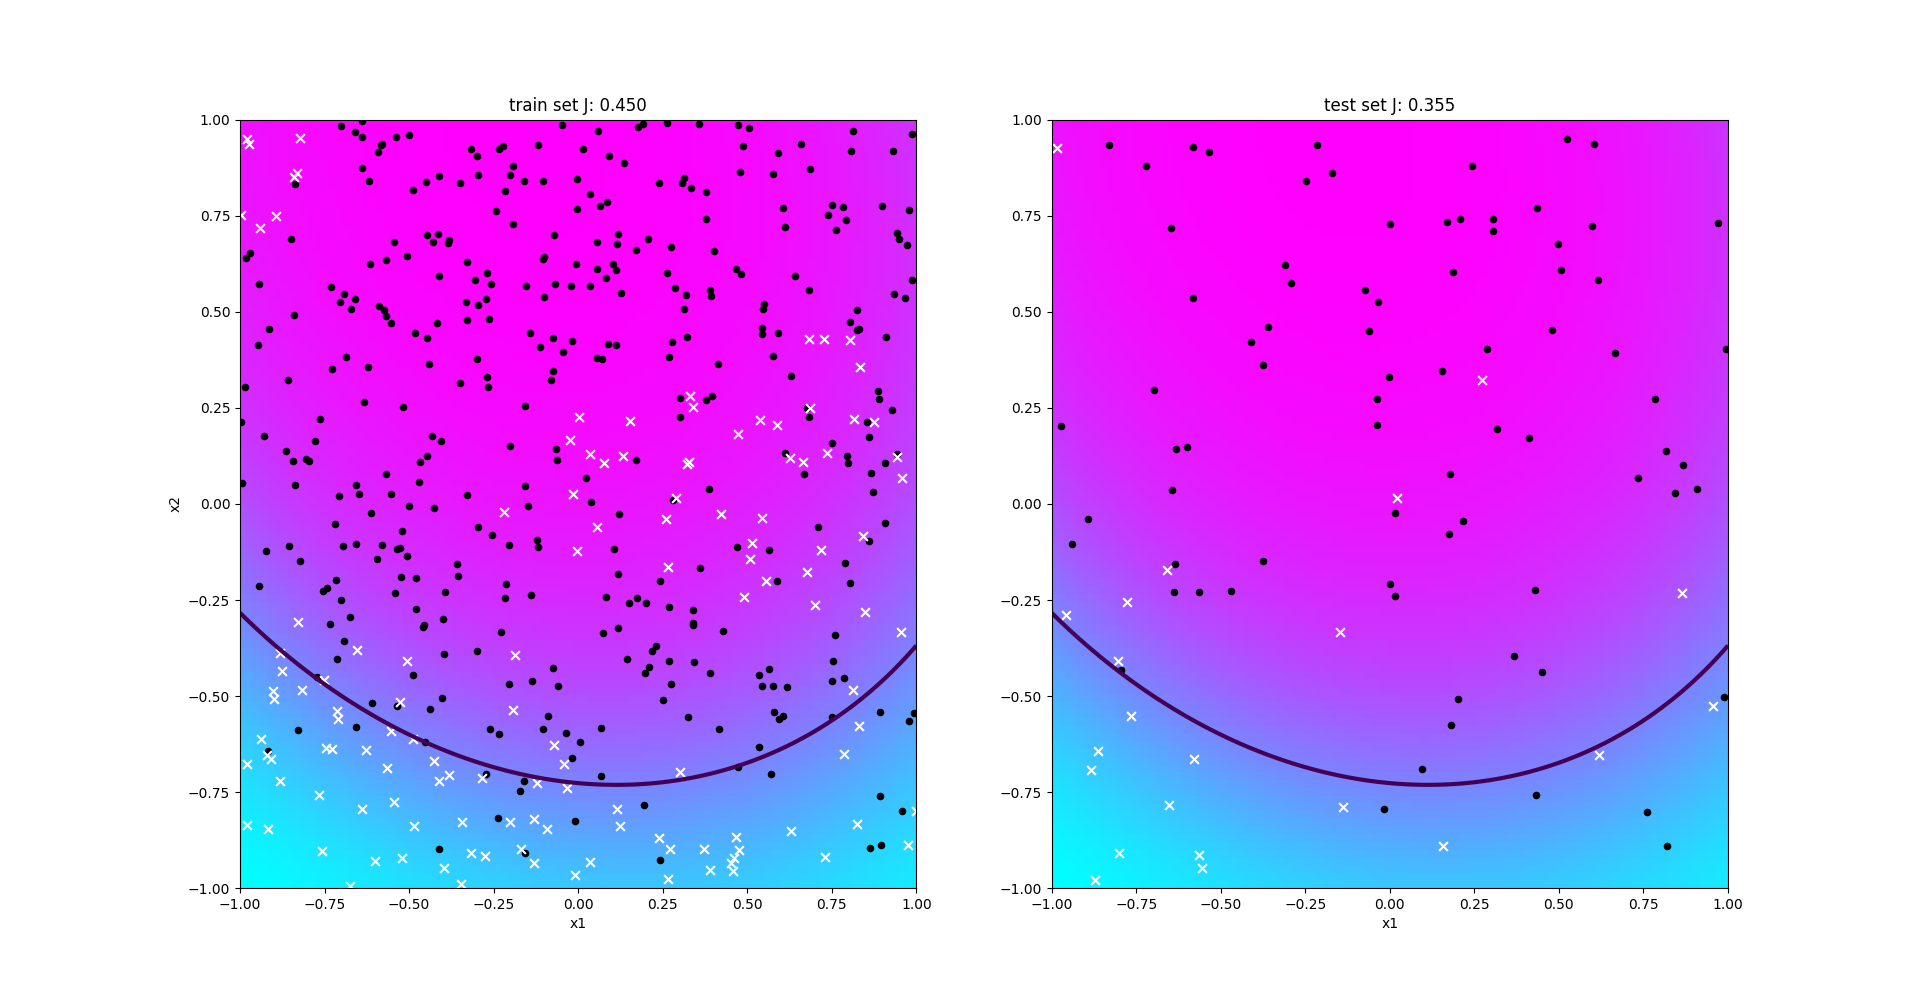
\includegraphics[width=\textwidth]{figures/logreg_d2_it200_15.png}
	    \caption{Logistic Regression ($\eta = 1.5$, $l = 1$, 200 iterations)}
	\end{figure}
	\begin{figure}[H]
  	\centering
	        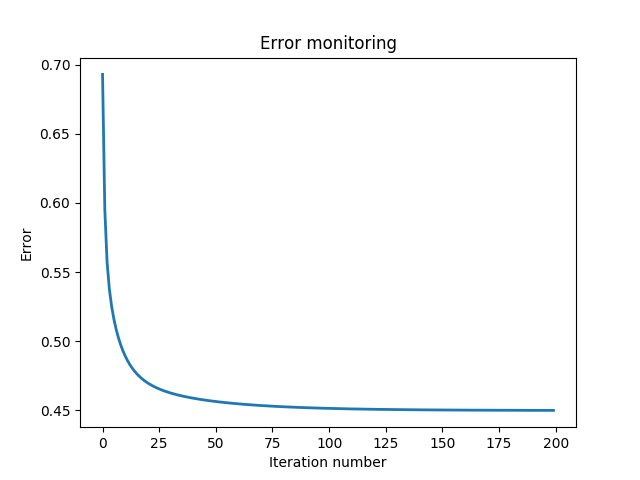
\includegraphics[width=\textwidth]{figures/logreg_d2_it200_15_error.png}
	    \caption{Logistic Regression Errors ($\eta = 1.5$, $l = 1$, 200
	    iterations)}
	\end{figure}
	\begin{figure}[H]
  	\centering
	        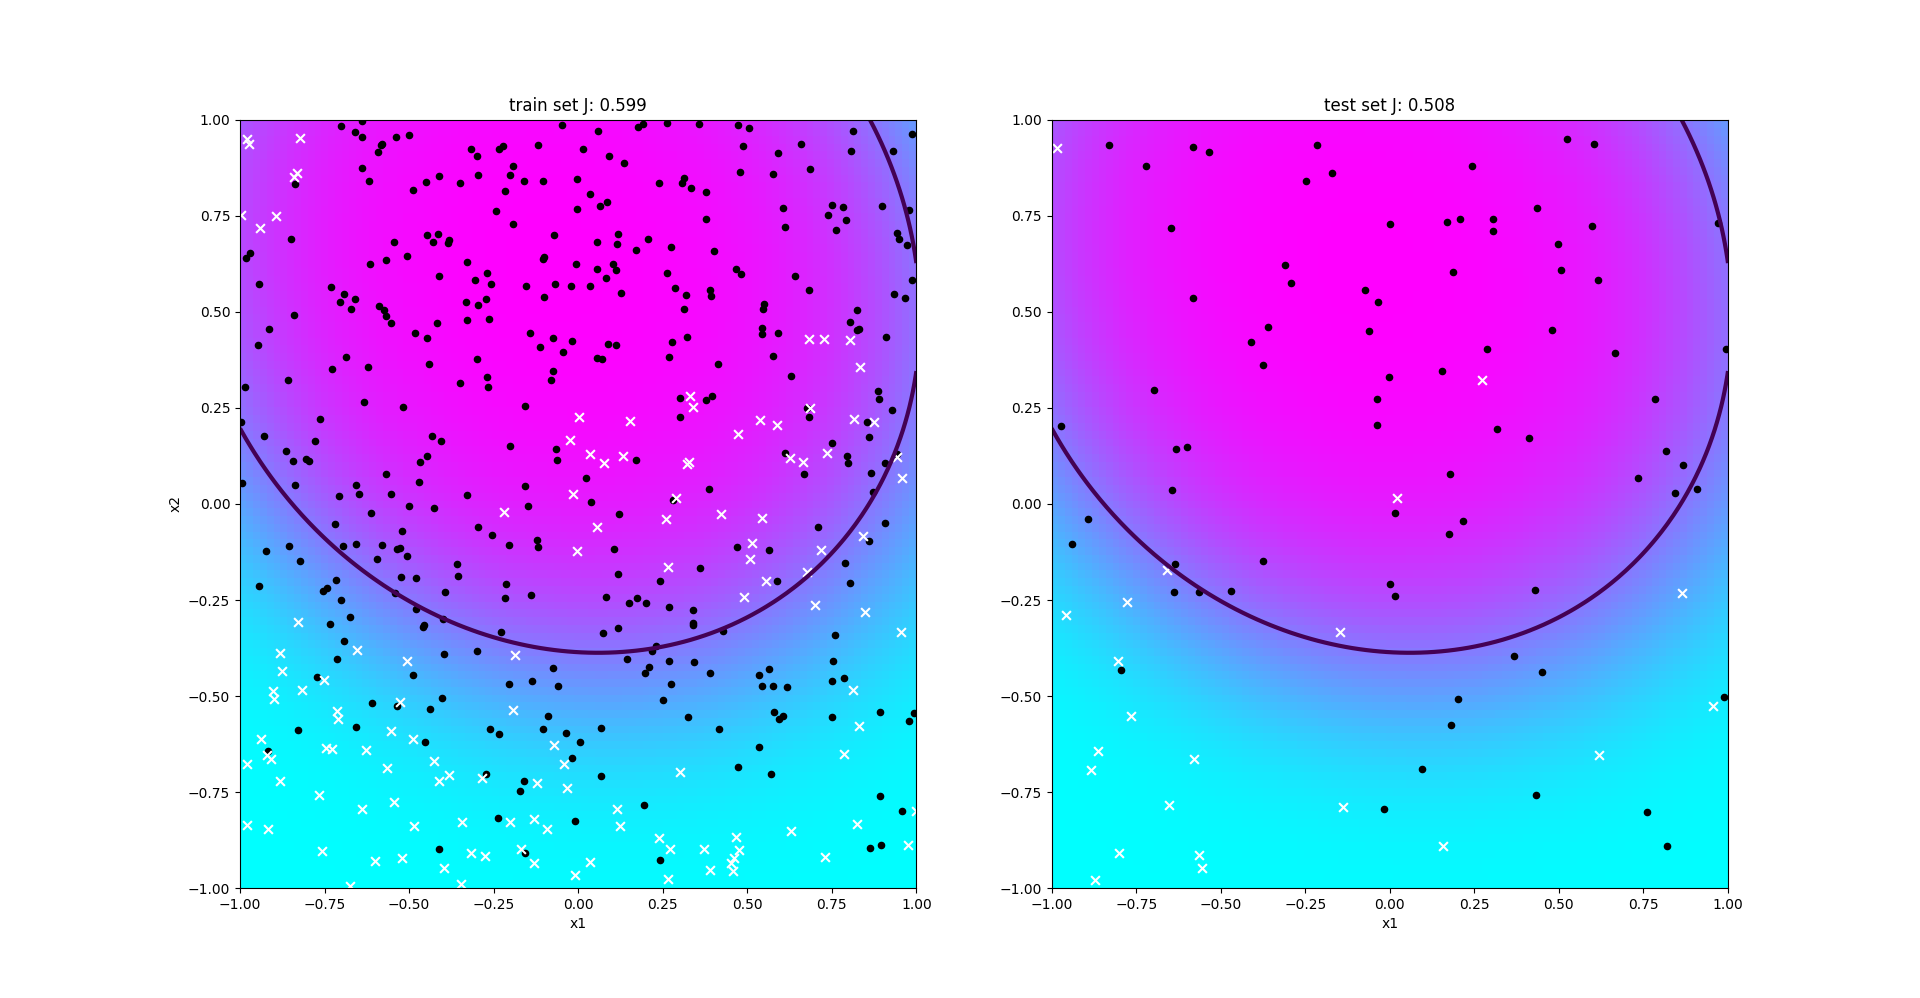
\includegraphics[width=\textwidth]{figures/logreg_d2_it200_15_.png}
	    \caption{Logistic Regression ($\eta = 15$, $l = 1$, 200 iterations)}
	\end{figure}
	\begin{figure}[H]
  	\centering
	        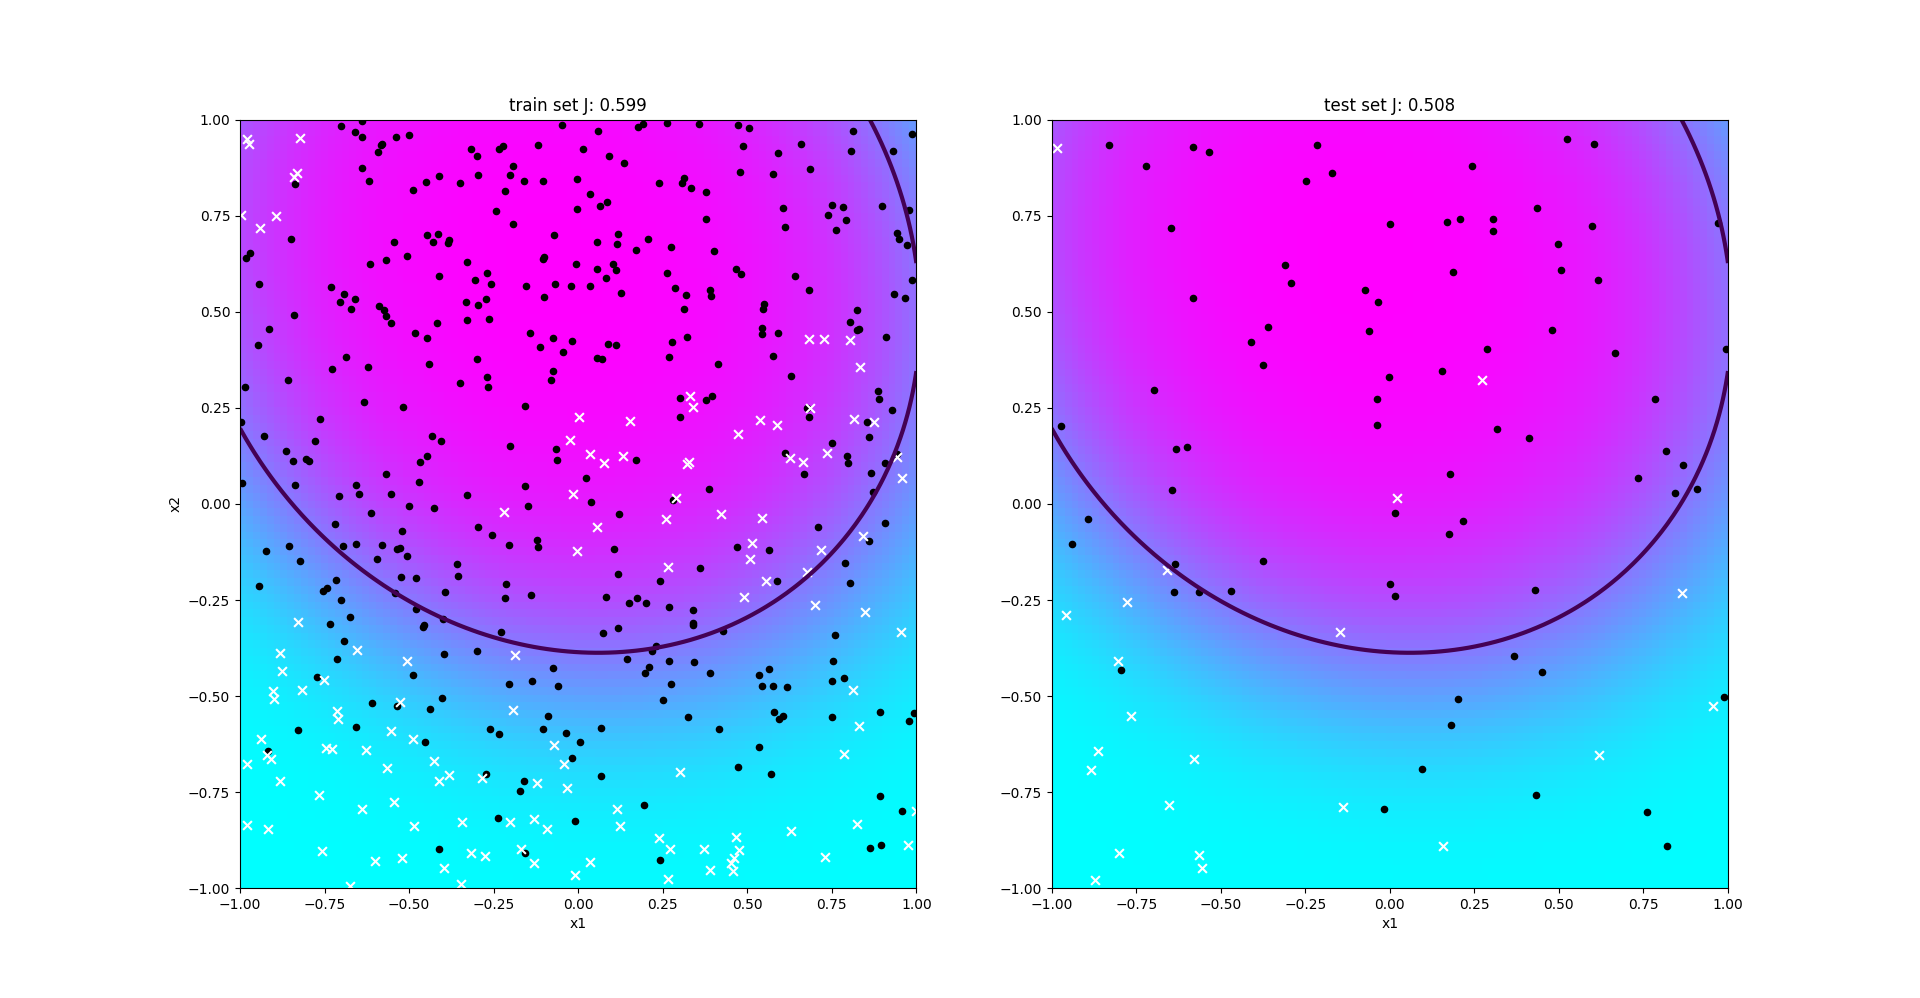
\includegraphics[width=\textwidth]{figures/logreg_d2_it200_15_.png}
	    \caption{Logistic Regression Errors ($\eta = 15$, $l = 1$, 200
	    iterations)}
	\end{figure}
	
	Discussion: Too low or too hight learning rates lead to divergence or spinning
	between lower and hight cost (oscillates).
	\item \textbf{Adaptative gradient descent (GDad)} degree $l
	= 1, 2, 5, 15$, 1000 iterations, learning rate $\eta = 1$
	\begin{figure}[H]
  	\centering
	        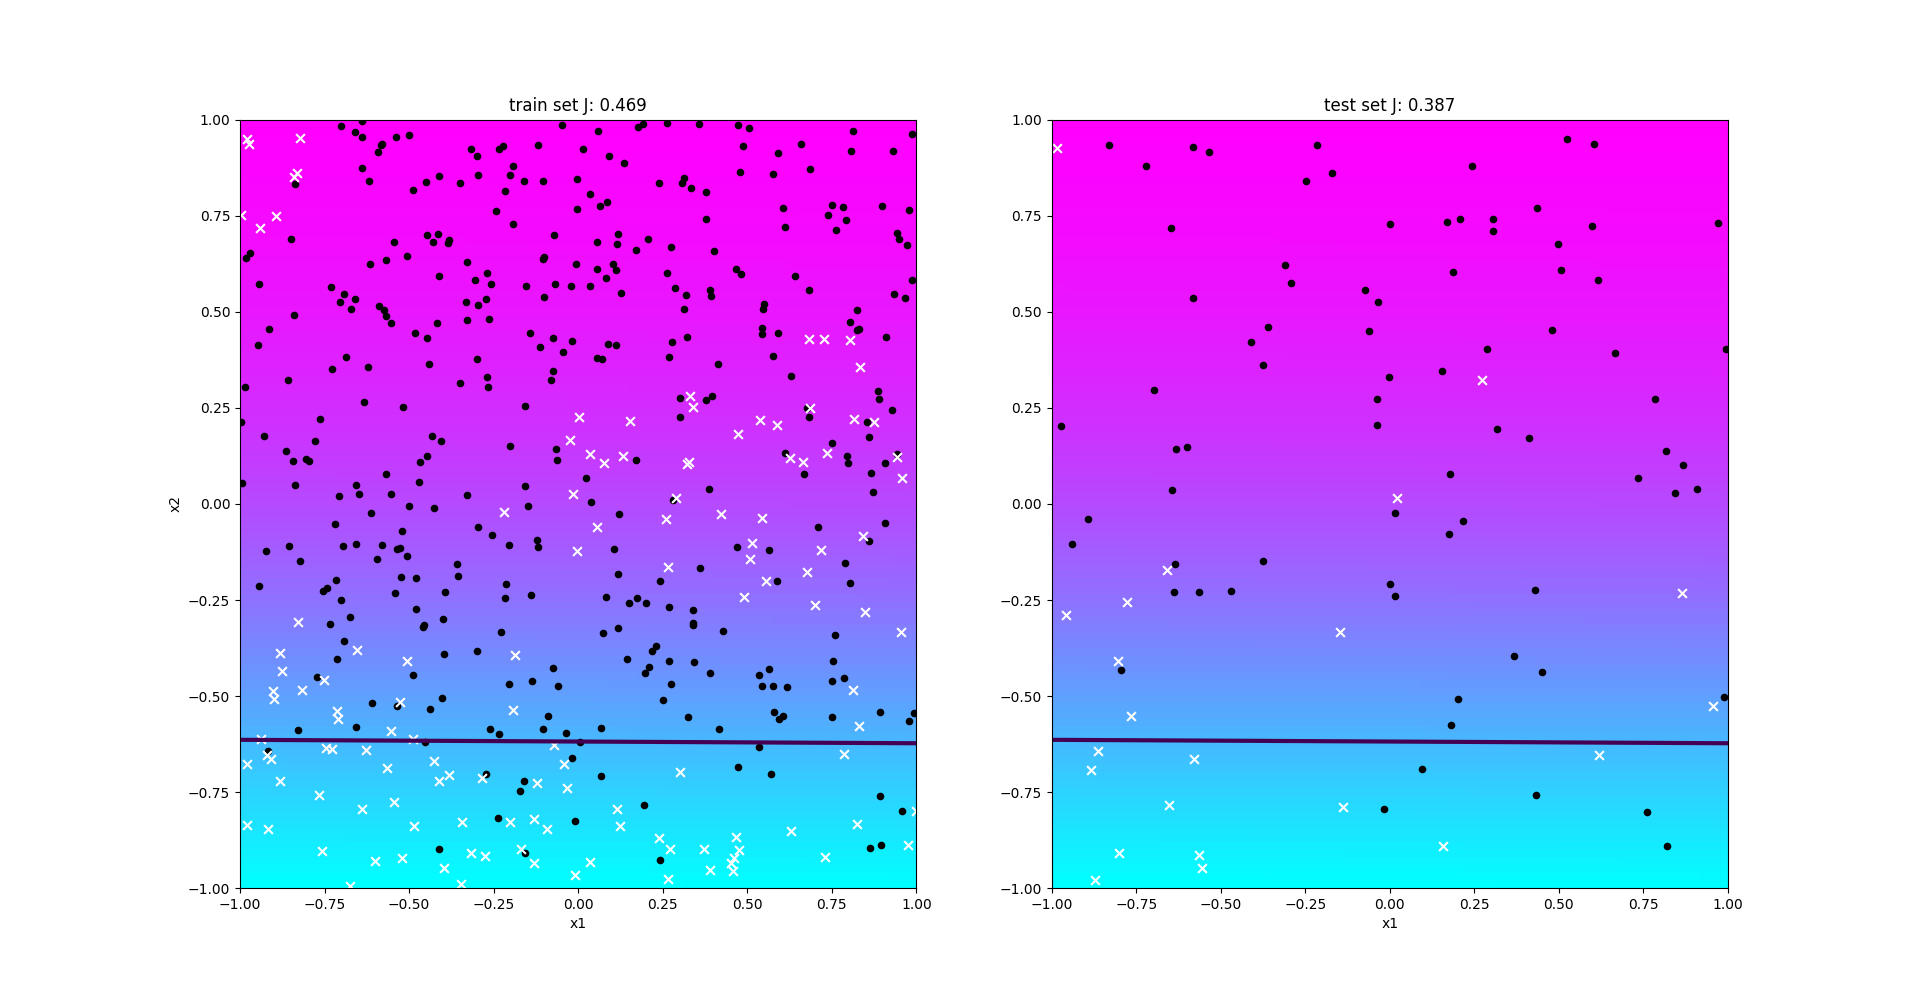
\includegraphics[width=\textwidth]{figures/logreg_adapt_1.png}
	    \caption{Logistic Regression (adaptive) ($\eta = 1$, $l = 1$, 1000
	    iterations)}
	\end{figure}
	\begin{figure}[H]
  	\centering
	        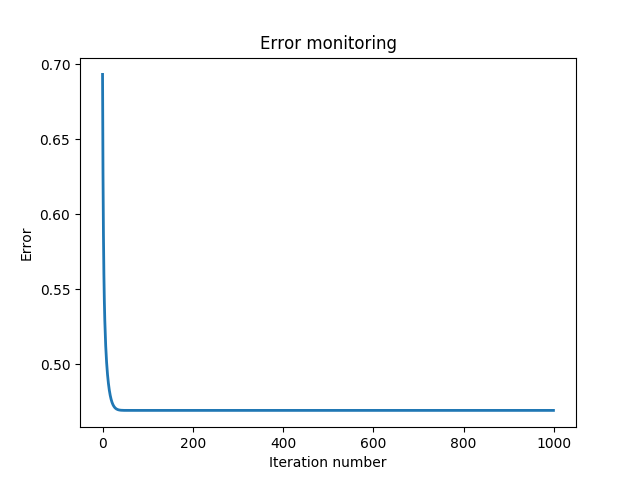
\includegraphics[width=\textwidth]{figures/logreg_adapt_1_error.png}
	    \caption{Logistic Regression (adaptive) Errors ($\eta = 1$, $l = 1$, 1000
	    iterations)}
	\end{figure}
	\begin{figure}[H]
  	\centering
	        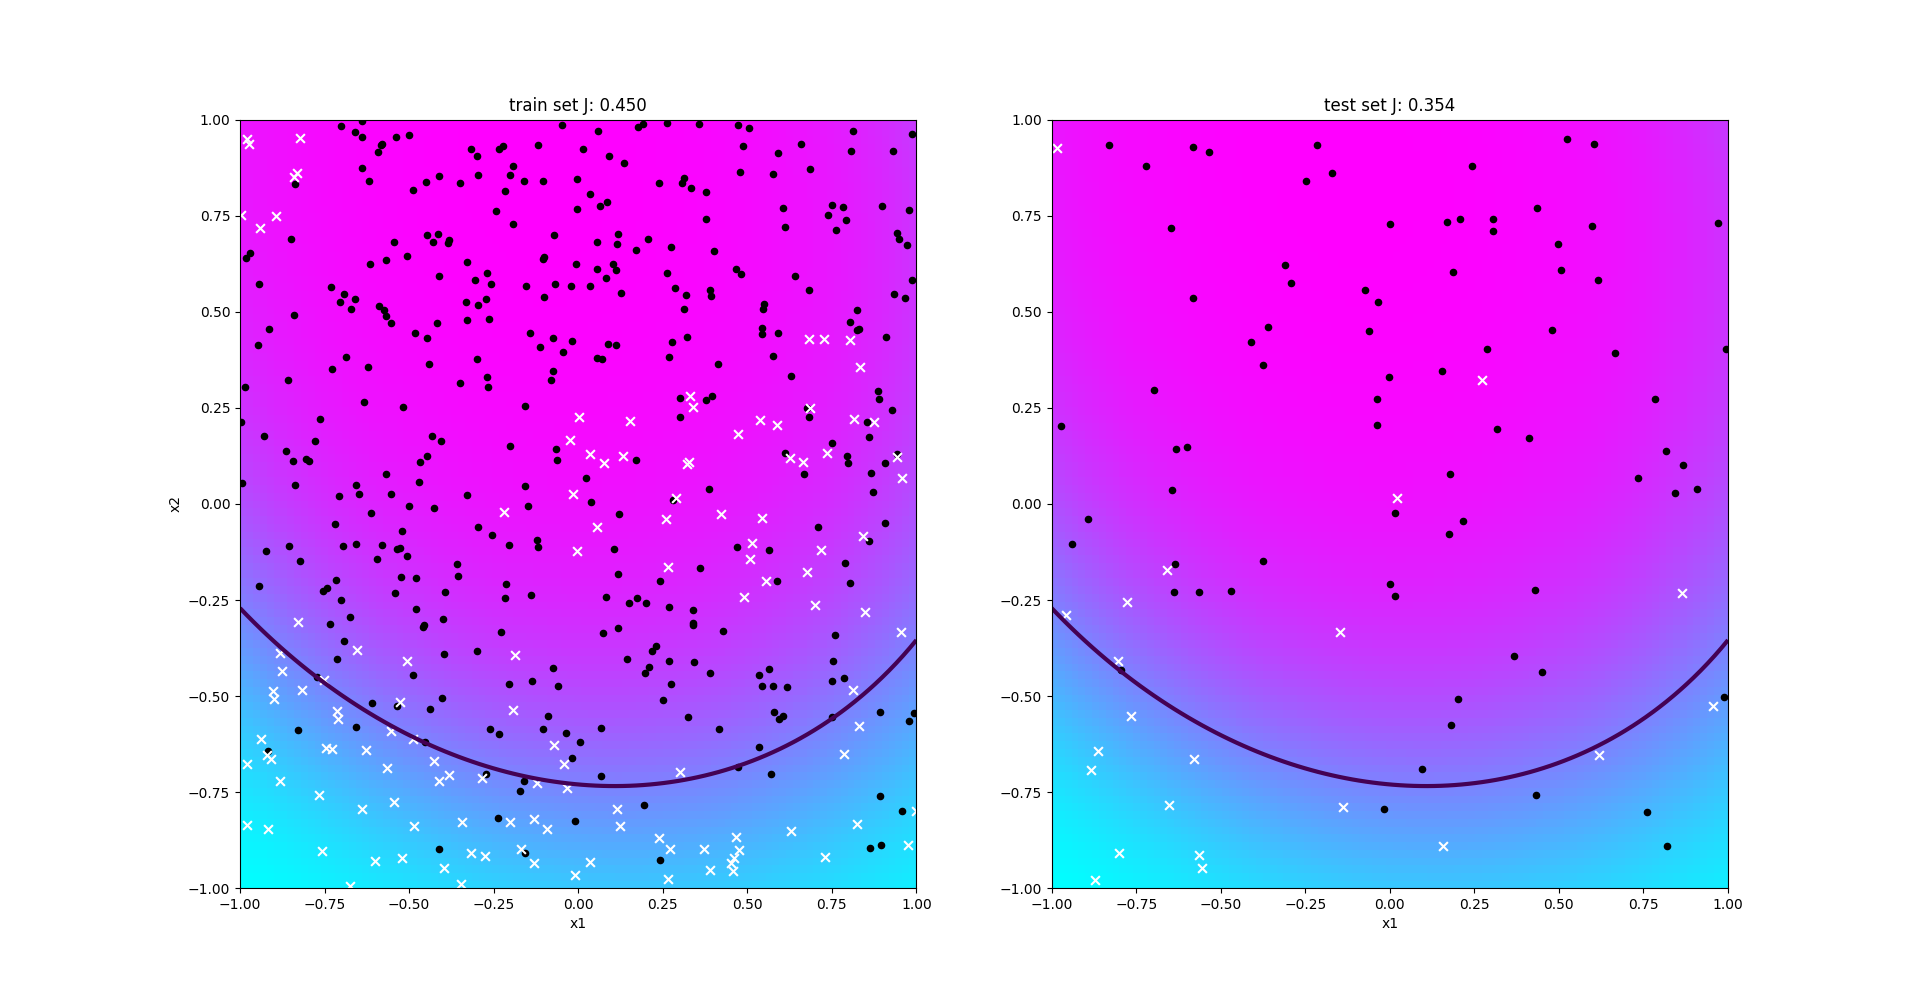
\includegraphics[width=\textwidth]{figures/logreg_adapt_2.png}
	    \caption{Logistic Regression (adaptive) ($\eta = 1$, $l = 2$, 1000
	    iterations)}
	\end{figure}
	\begin{figure}[H]
  	\centering
	        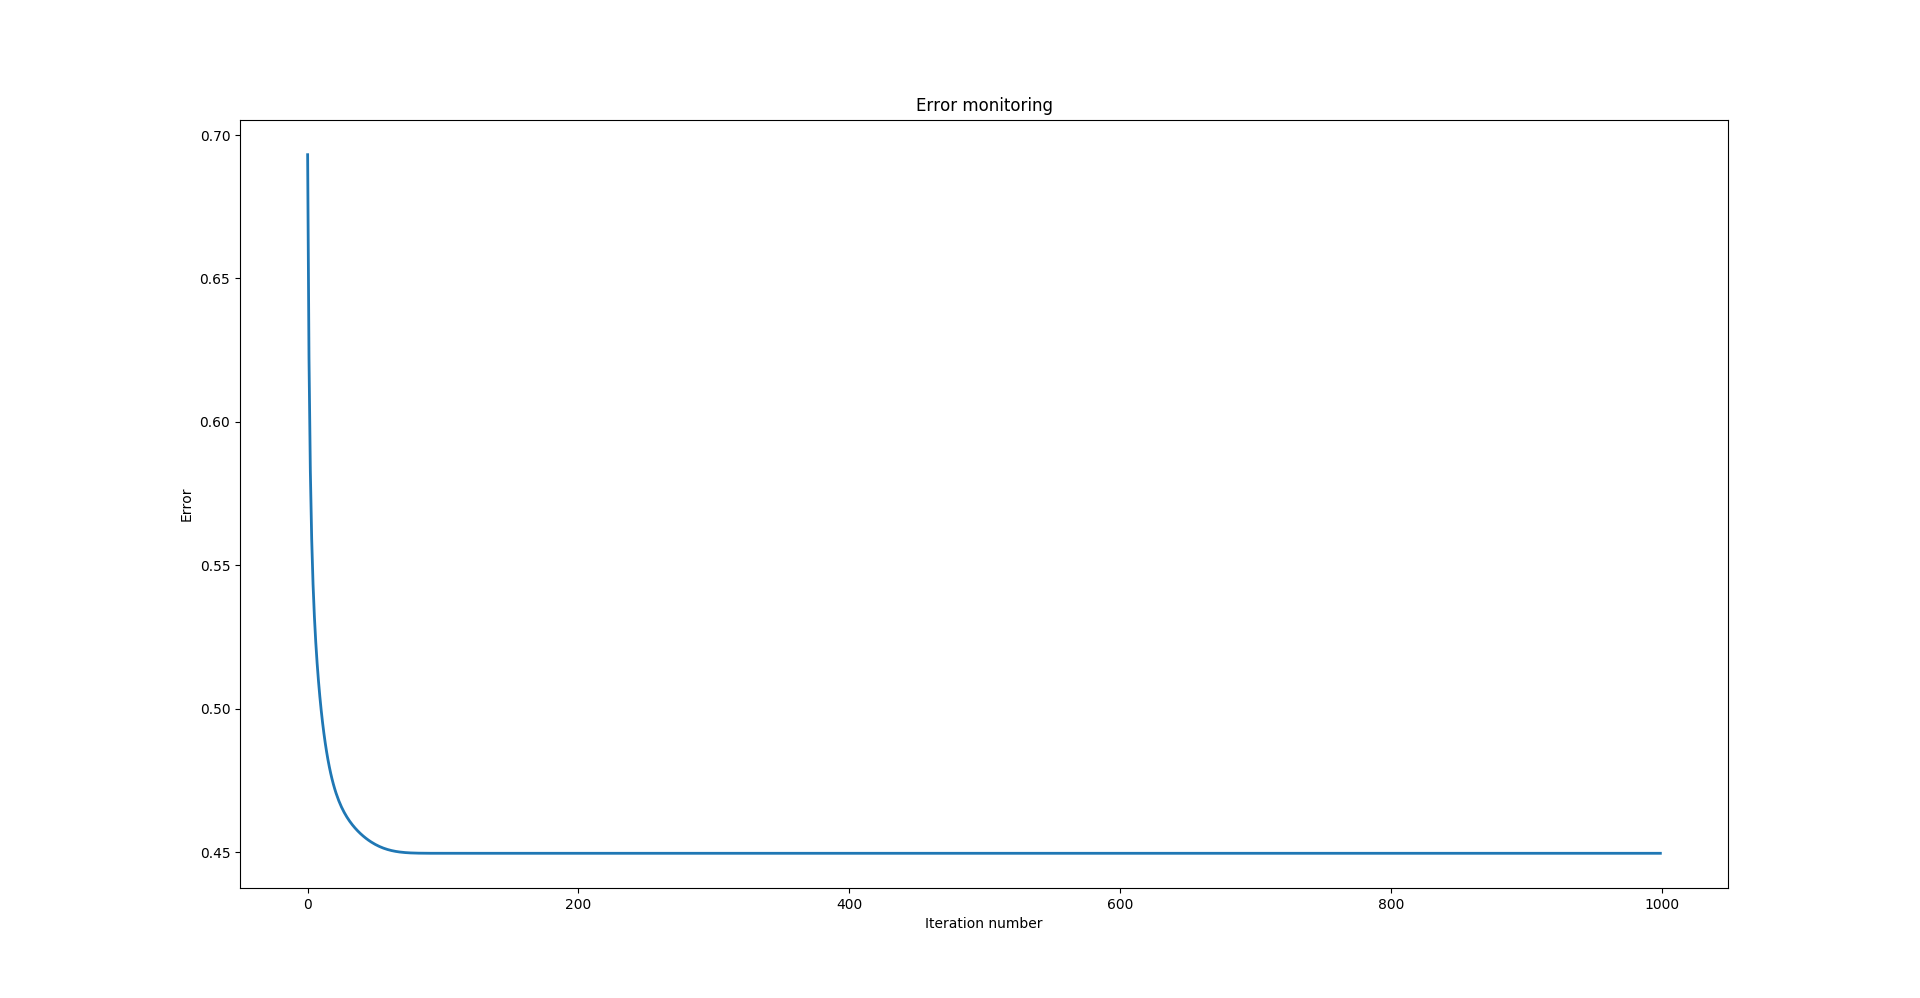
\includegraphics[width=\textwidth]{figures/logreg_adapt_2_error.png}
	    \caption{Logistic Regression (adaptive) Errors ($\eta = 1$, $l = 2$, 1000
	    iterations)}
	\end{figure}
	\begin{figure}[H]
  	\centering
	        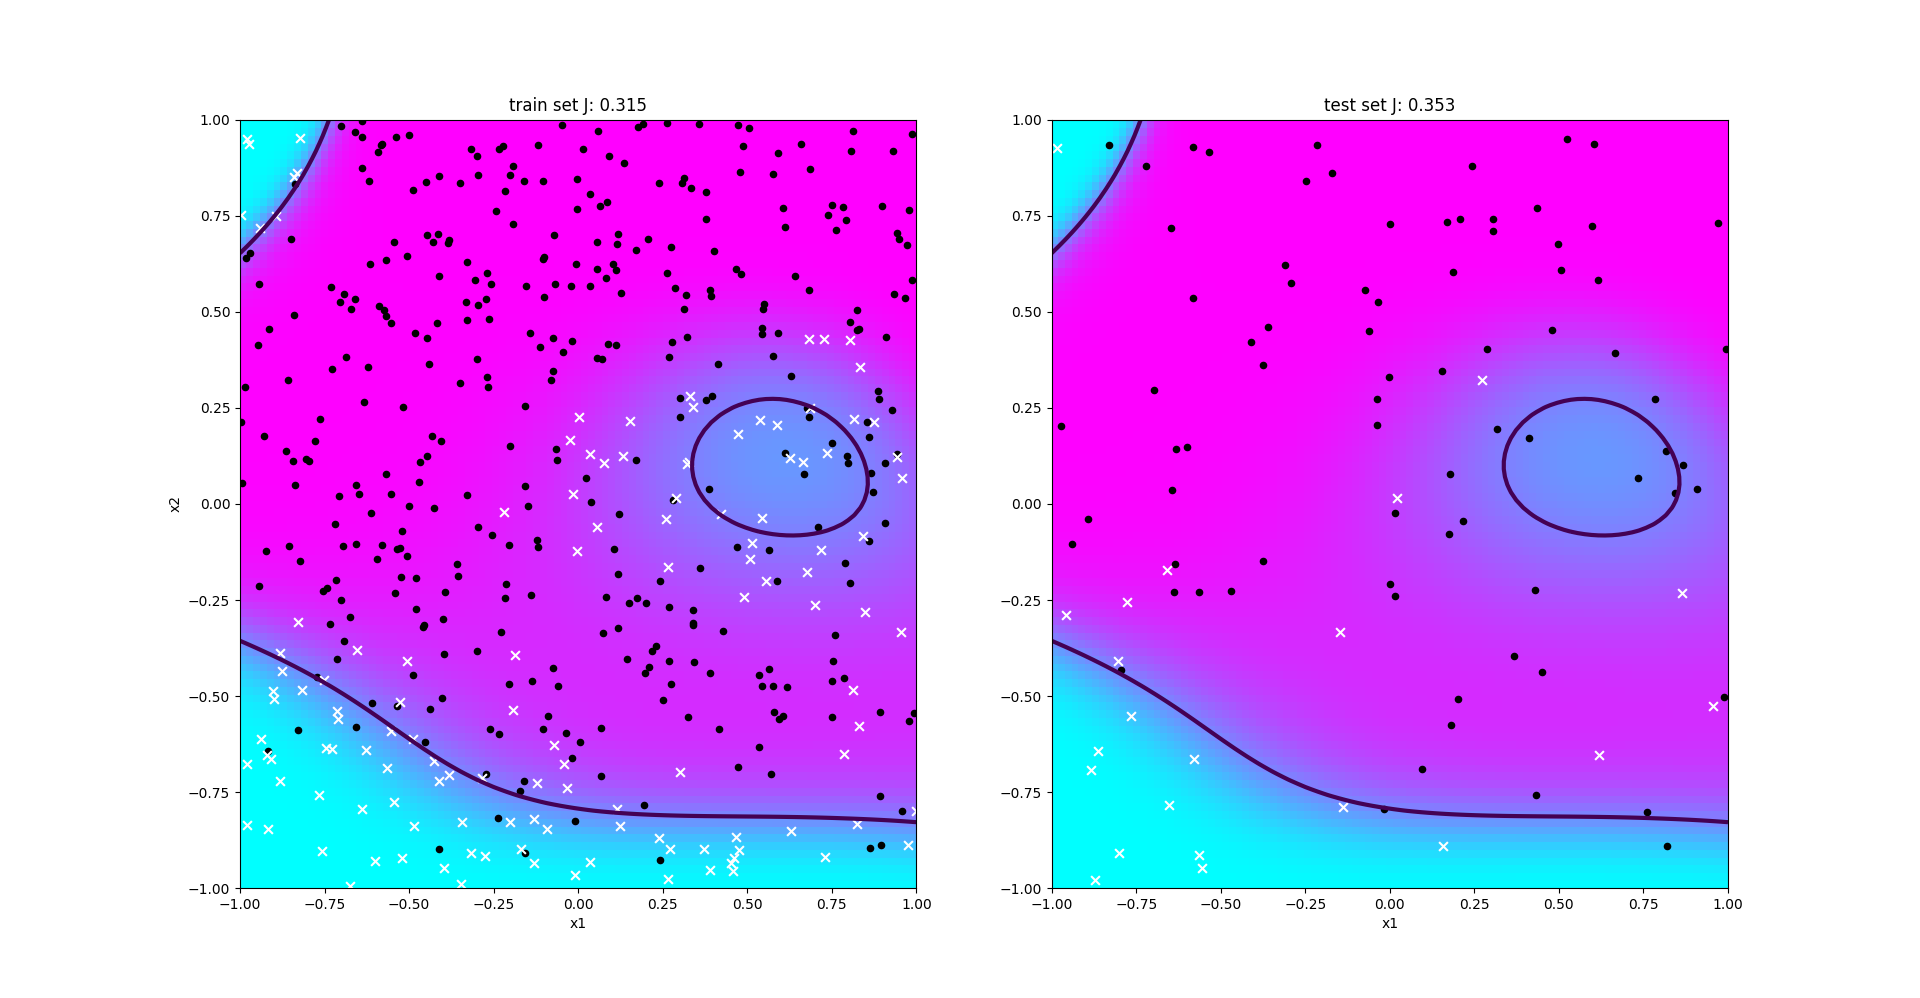
\includegraphics[width=\textwidth]{figures/logreg_adapt_5.png}
	    \caption{Logistic Regression (adaptive) ($\eta = 1$, $l = 5$, 1000
	    iterations)}
	\end{figure}
	\begin{figure}[H]
  	\centering
	        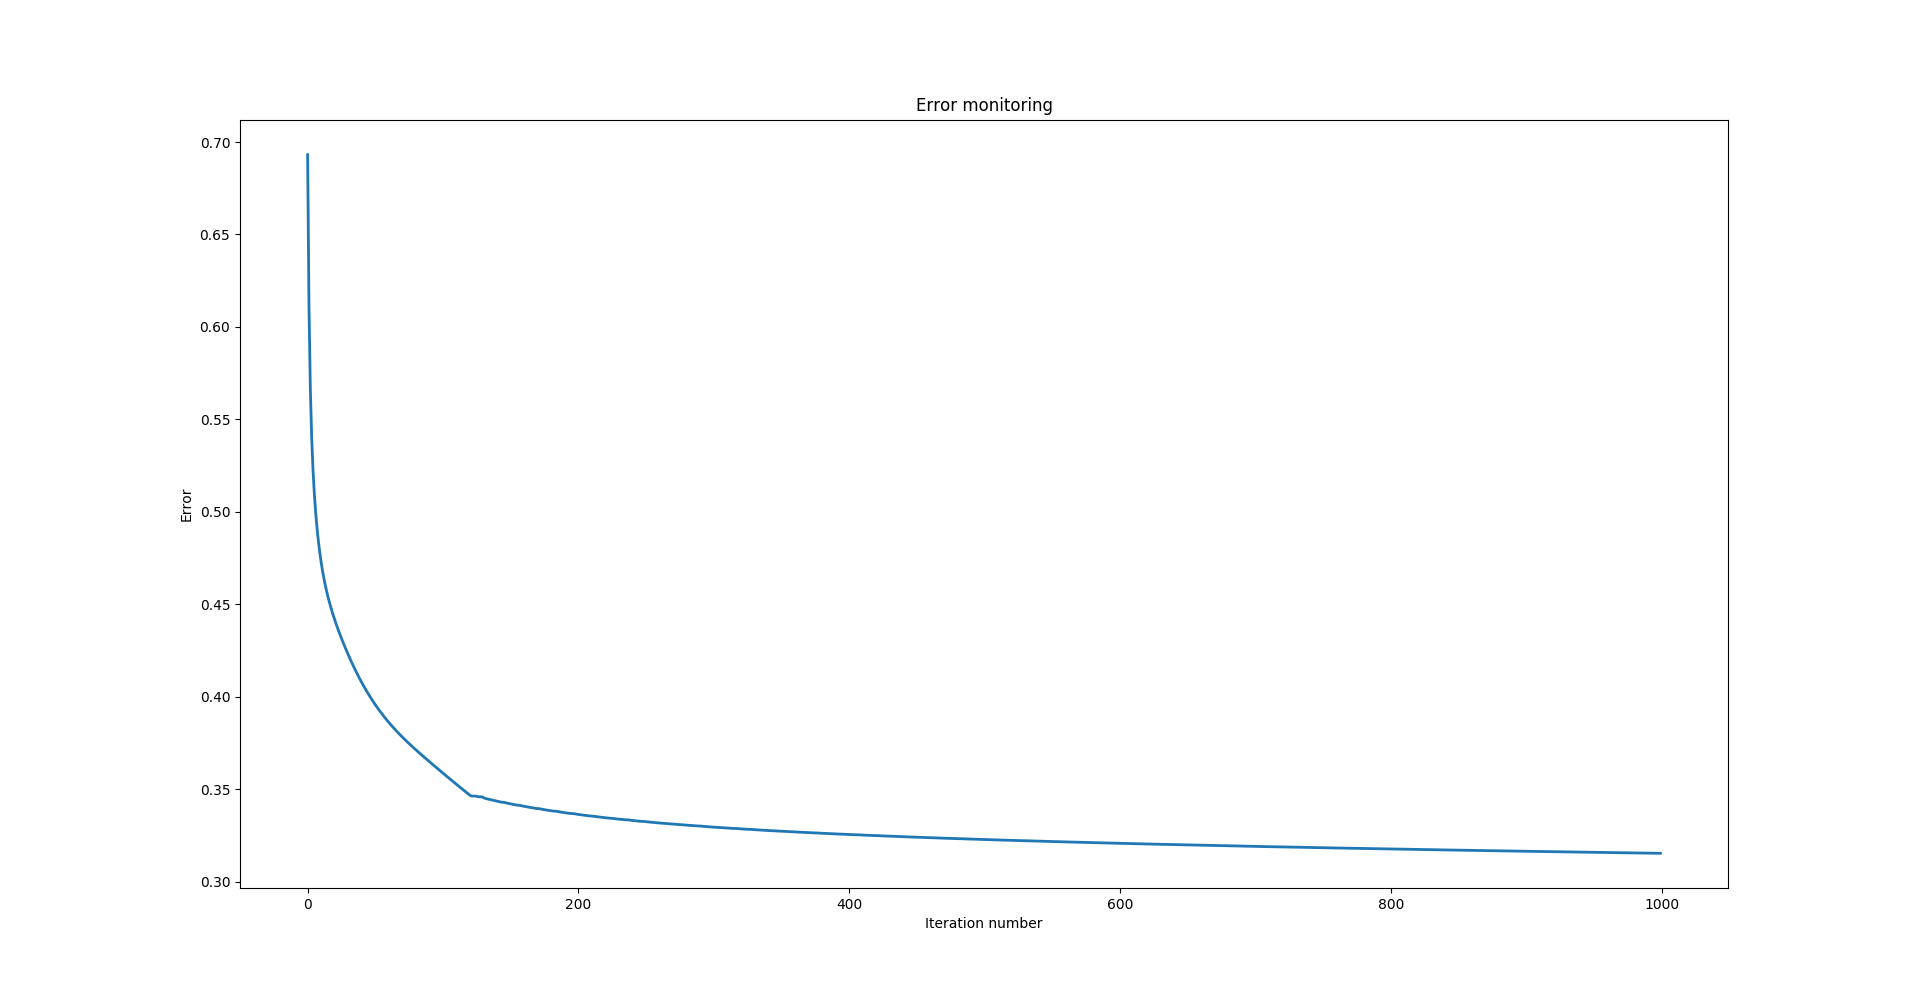
\includegraphics[width=\textwidth]{figures/logreg_adapt_5_error.png}
	    \caption{Logistic Regression (adaptive) Errors ($\eta = 1$, $l = 5$, 1000
	    iterations)}
	\end{figure}
	\begin{figure}[H]
  	\centering
	        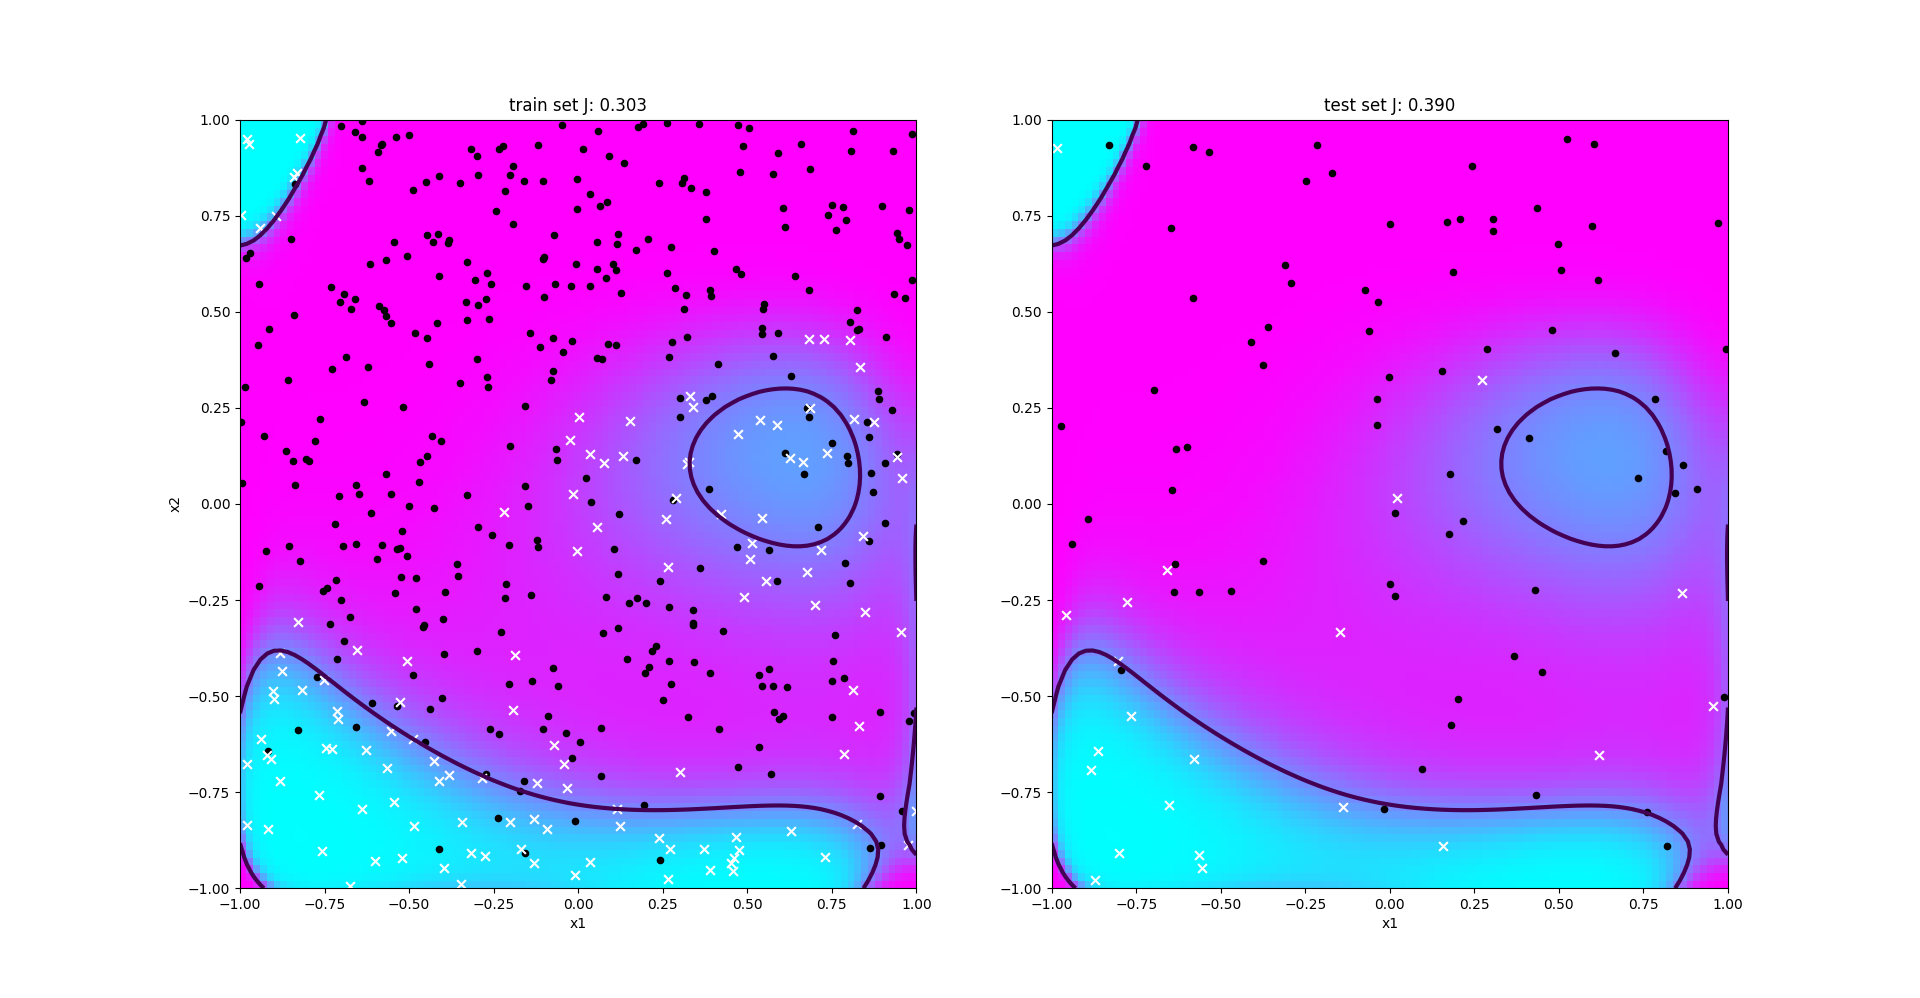
\includegraphics[width=\textwidth]{figures/logreg_adapt_15.png}
	    \caption{Logistic Regression (adaptive) ($\eta = 1$, $l = 15$, 1000
	    iterations)}
	\end{figure}
	\begin{figure}[H]
  	\centering
	        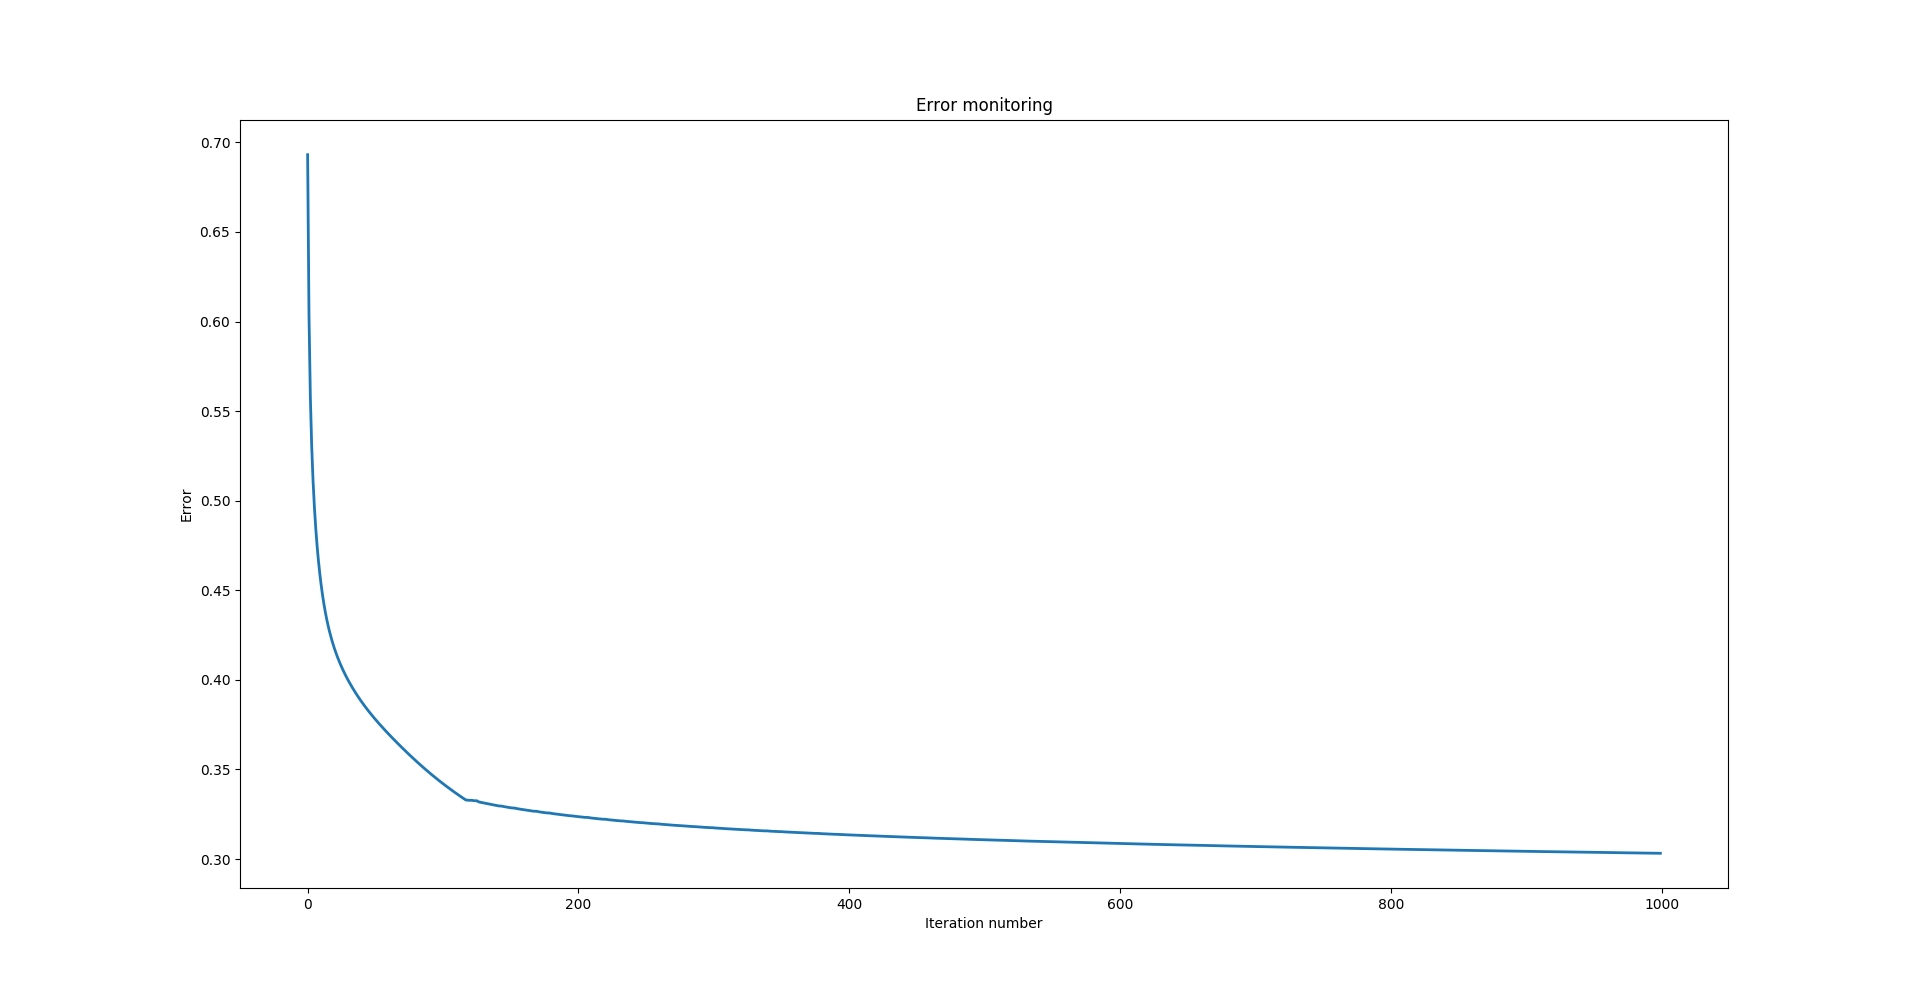
\includegraphics[width=\textwidth]{figures/logreg_adapt_15_error.png}
	    \caption{Logistic Regression (adaptive) Errors ($\eta = 1$, $l = 15$, 1000
	    iterations)}
	\end{figure}
	\item Stopping
	When error between iteration becomes too low, threshold regression should be
	stopped.
\end{enumerate}


\subsubsection{Scipy optimizer}

\end{document}